%
% Chapter 9
%

\chapter{SIGNAL EXTRACTION}
\label{chap:extraction}
The signal extraction procedure is the method by which a suitable variable, which discriminates signal
from background, is selected and binned. Then, separate counting experiments are performed in each
resulting bin. The collection of these counting experiments is then used to produce the final
result, the measurement of \tth signal process. This method is executed in the signal region, and offers
a distinct advantage with respect to a ``cut-and-count'' procedure where no discriminant is used and 
a single counting experiment is performed in the signal region.
By dividing the signal region into bins of a discriminant, each bin has a unique
signal to background ratio, with some bins having a significantly higher signal to background ratio
than others. The motivation for the signal extraction procedure is that the geometric average of the
signal to background ratios of the bins of the discriminant is higher than the signal to background ratio
obtained with the signal counting experiment in the cut-and-count method. 

The discriminant used to separate signal from background is based on a multivariate analysis algorithm 
called a Boosted Decision Tree (BDT). The BDT discriminant combines information from several input discriminating
variables into a single variable more powerful than any single input. 
The composition of signal and background predictions, as well as data, in the signal region where the
signal extraction is performed is in Table~\ref{tab:yields} below.

\begin{table}[htbp]
\begin{center}
  \caption[Signal region event yields by lepton flavor]{Expected (pre-fit) yields for signal and background processes, and observed yields in data. Uncertainties shown
are purely statistical.}
    \begin{tabular}{l c c c} \hline
& $\mu\mu$ & $ee$ & $e\mu$  \\ \hline 
$t\bar{t}W$ & 45.4 $\pm$ 0.5 & 17.8 $\pm$ 0.3 & 64.3 $\pm$ 0.6 \\
$t\bar{t}Z/\gamma^{*}$ & 16.8 $\pm$ 0.7 & 14.8 $\pm$ 0.8 & 41.7 $\pm$ 1.4 \\
\hline
WZ & 5.2 $\pm$ 0.7 & 1.6 $\pm$ 0.4 & 7.5 $\pm$ 0.8 \\
Rare SM. bkg & 6.8 $\pm$ 0.3 & 3.5 $\pm$ 0.2 & 11.7 $\pm$ 0.4 \\
WWss & 2.9 $\pm$ 0.2 & 1.4 $\pm$ 0.1 & 4.3 $\pm$ 0.2 \\
\hline
Conversions & 0.0 $\pm$ 0.0 & 3.4 $\pm$ 1.1 & 8.5 $\pm$ 1.3 \\
Charge flip & 0.0 $\pm$ 0.0 & 172 $\pm$ 93 & 149 $\pm$ 82 \\
Non-prompt leptons & 29.9 $\pm$ 1.2 & 17.3 $\pm$ 1.1 & 53.5 $\pm$ 1.8 \\
\hline
Total bkg & 107.3 $\pm$ 1.7 & 70.3 $\pm$ 1.8 & 208.0 $\pm$ 2.9 \\
 \hline
$t\bar{t}H$ & 18.5 $\pm$ 0.2 & 7.4 $\pm$ 0.1 & 26.2 $\pm$ 0.2 \\
 \hline
Data & 154 & 95 & 274 \\
\hline
\end{tabular}
    \label{tab:yields}
\end{center}
\end{table}

The signal extraction strategy adopted here targets the two largest backgrounds, \ttv and the non-prompt leptons, using separate BDTs to discriminate against each
specific background. The inputs to these BDTs include kinematic variables, as well as outputs of other BDTs designed to resconstruct parts of the signal
events such as the Higgs jets and the hadronically decaying top quark. Finally, the outputs of the BDT dscriminators are plotted on separate axes forming a two-dimensional
distribution, referred to here as the 2D BDT. This shape is then binned in two dimensions forming a one-dimensional discriminant. 

\section{Two Dimensional BDTs}
\label{sec:2D_BDT}
Two BDTs are used to produce the final shape template. One BDT is trained exclusively against the \ttv background, while the other targets the background due to non-prompt
leptons. The BDT descriminating against the non-prompt lepton background is trained against \ttbar MC, since the \ttbar processes is the largest source of non-prompt leptons.
The BDT that discriminates against \ttv is trained against \ttw and \ttz MC events. The MC samples used for BDT training are separate from the samples used in the final
analysis which is a standard practice when using MVA discriminants. Using independent training samples is necessary to avoid biasing the MVA analysis. 

A loosened version of the $2lss$ signal region selection is applied to the MC samples used for training. This loosened selection is motivated by increasing the training statistics available
while not affecting the behavior and kinematics of the input variables with respect to the signal region. This loosened selection consists of the following criteria:
\begin{itemize}
\item At least two preselected same-sign leptons
\item The lepton \pt $>$ 25,15 
\item At least 4 preselected jets among which there must be $\geq$ 2 CSVv2 L or $\geq$ 1 CSVv2 M
\end{itemize}

Many BDT input variables were tested, and the set of variables which produced the most discriminating BDT output was selected. These inputs are listed in Table~\ref{tab:inputs}.
Selecting which variables to use as inputs requires several considerations. First, since the BDTs are trained on MC and ultimately evaluated on data, every
input variable must be well-modeled, i.e. have a good agreement between MC and data. Second, the candidate inputs, at least some, should have signal separation power themselves,
which allows the BDT to learn this information. The final consideration is more subtle. While the separation power of individal inputs is important, selecting each input
based on its separation does not necessarily produce the most discriminating BDT. Correlations can exist between different variables, and if these correlations exist in
signal and background, the BDT does not learn additional information from these correlated variables. However, if two variables are correlated differently in signal
than in background, the BDT makes use of this in separating signal from background. All these considerations were taken into account when empirically determining the best
set of BDT inputs.

\begin{table}[htbp]
  \begin{center}
  \caption[Table of 2D BDT input variables]{Input variables used for the BDTs targeting \ttbar and \ttv.}
  \begin{tabular}{|p{0.47\textwidth}|p{0.47\textwidth}|} \hline
    \multicolumn{1}{|c|}{\ttbar} & \multicolumn{1}{c|}{\ttv}  \\ 
    \hline 
    \multicolumn{2}{|c|}{Maximum absolute $\eta$ of the two leptons (max lepton $|\eta|$)}  \\
    \hline
    \multicolumn{2}{|c|}{Number of hadronic jets (nJets)} \\
    \hline
    \multicolumn{2}{|c|}{Minimum $\Delta$R between the leading lepton and nearest jet}\\
    \hline
    \multicolumn{2}{|c|}{Minimum $\Delta$R between the trailing lepton and nearest jet}\\
    \hline
    \multicolumn{2}{|c|}{Transverse mass of the leading lepton and \met ($M_{T}$(\met,$lep_{1}$))} \\
    \hline
    The hadronic top reconstruction score & The Higgs jet tagger score after hadronic top removal \\
    \hline
    - & The leading lepton corrected transverse momentum  \\
    \hline
    - & The trailing lepton corrected transverse momentum  \\
    \hline
  \end{tabular}
  \label{tab:inputs}
  \end{center}
\end{table}


\noindent The hadronic top reconstruction score and the Higgs jet tagger score are outputs of separate event reconstruction BDTs, which aim to match jets
to the hadronically decaying top quark and the hadronically decaying daughter of the Higgs respectively. These BDT outputs provide
discriminating input variables to the 2D BDT. The details of these reconstruction BDTs are described in the following subsections.  
The 2D BDT input variable distributions of \tth, \ttbar, and \ttv are in Figures~\ref{fig:inputs1},~\ref{fig:inputs2},~\ref{fig:inputs3}.
The distributions are normalized to equal area to visualize separation between signal and background. 
For details on the training of all BDTs described in this section, as well as a description of the BDT technique itself, see Appendix~\ref{app:bdts}.

\begin{figure}[htp]
\centering
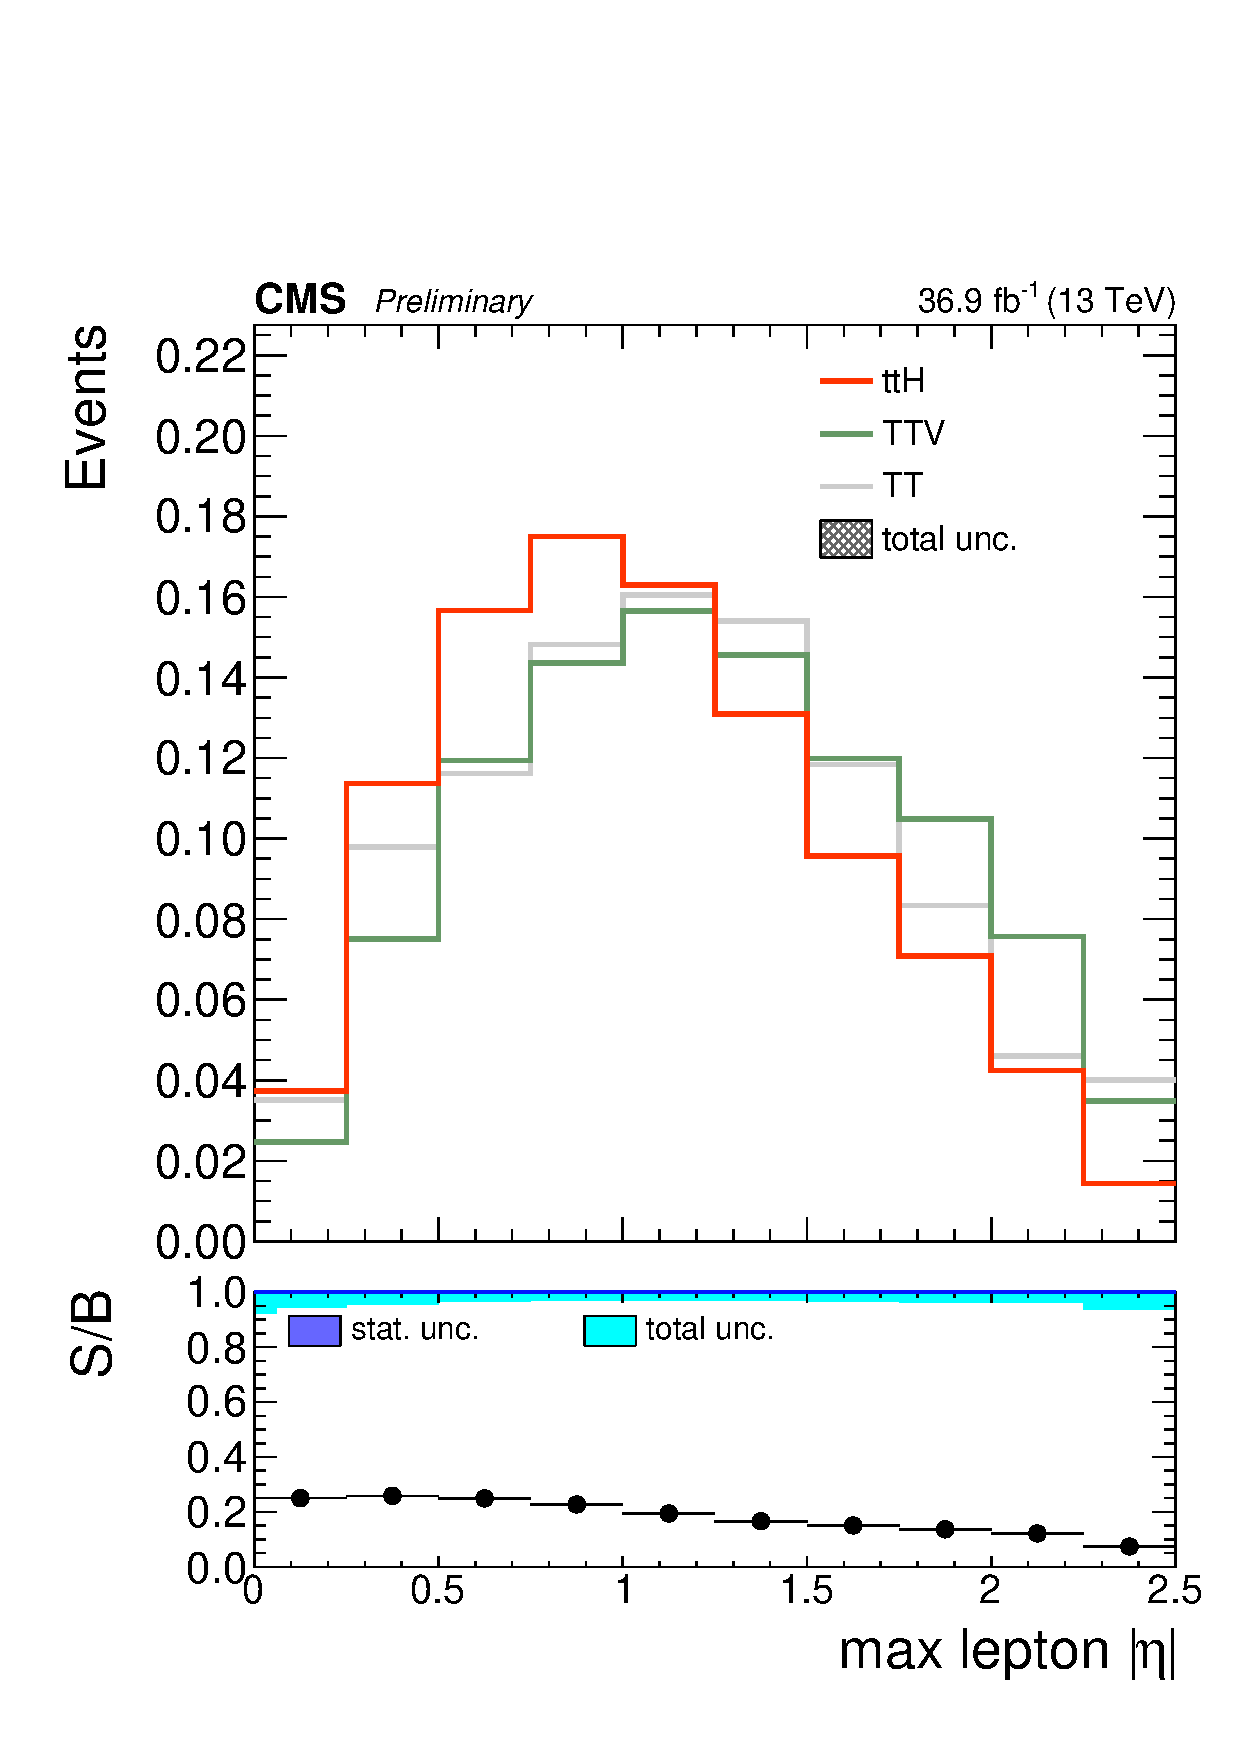
\includegraphics[width=0.3\textwidth]{ch9_figs/kinMVA_input_max_Lep_eta.pdf}
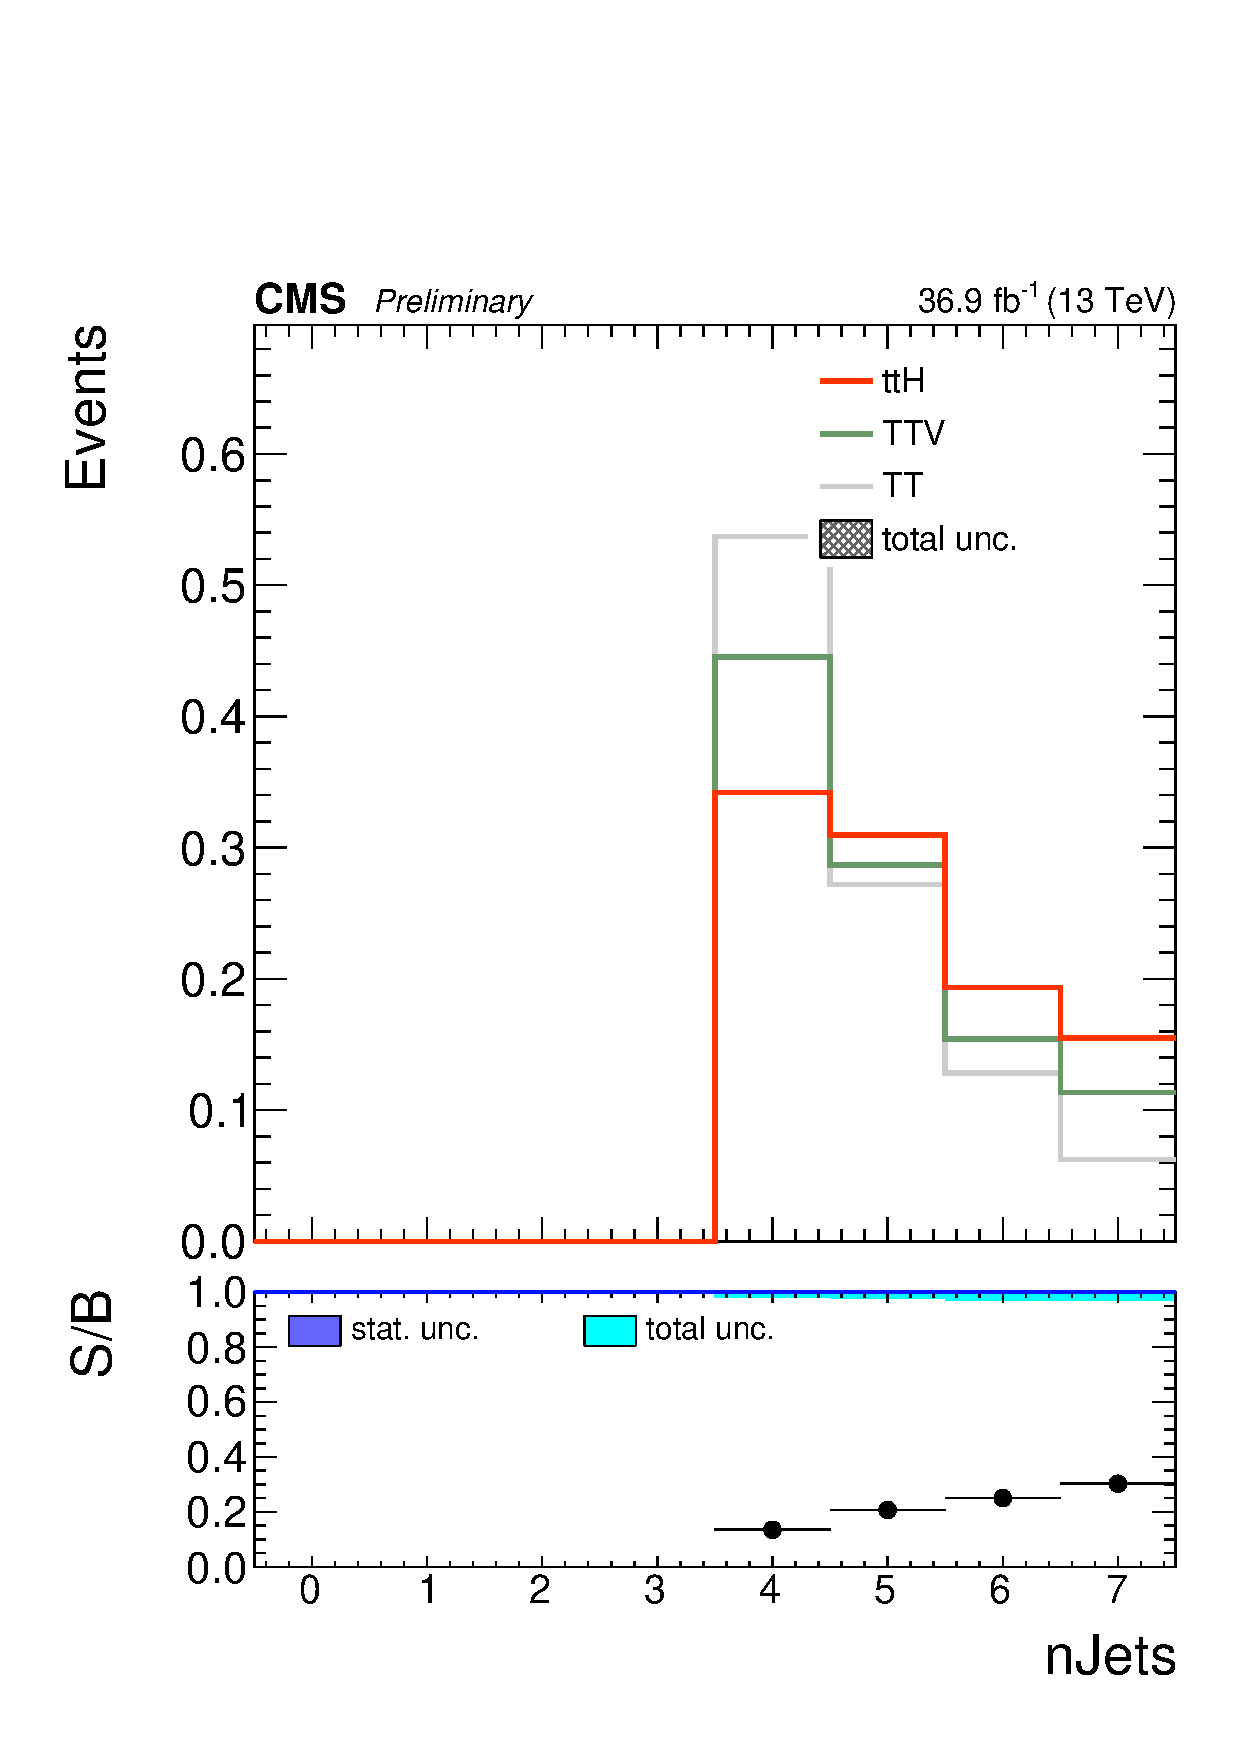
\includegraphics[width=0.3\textwidth]{ch9_figs/kinMVA_input_numJets.pdf}
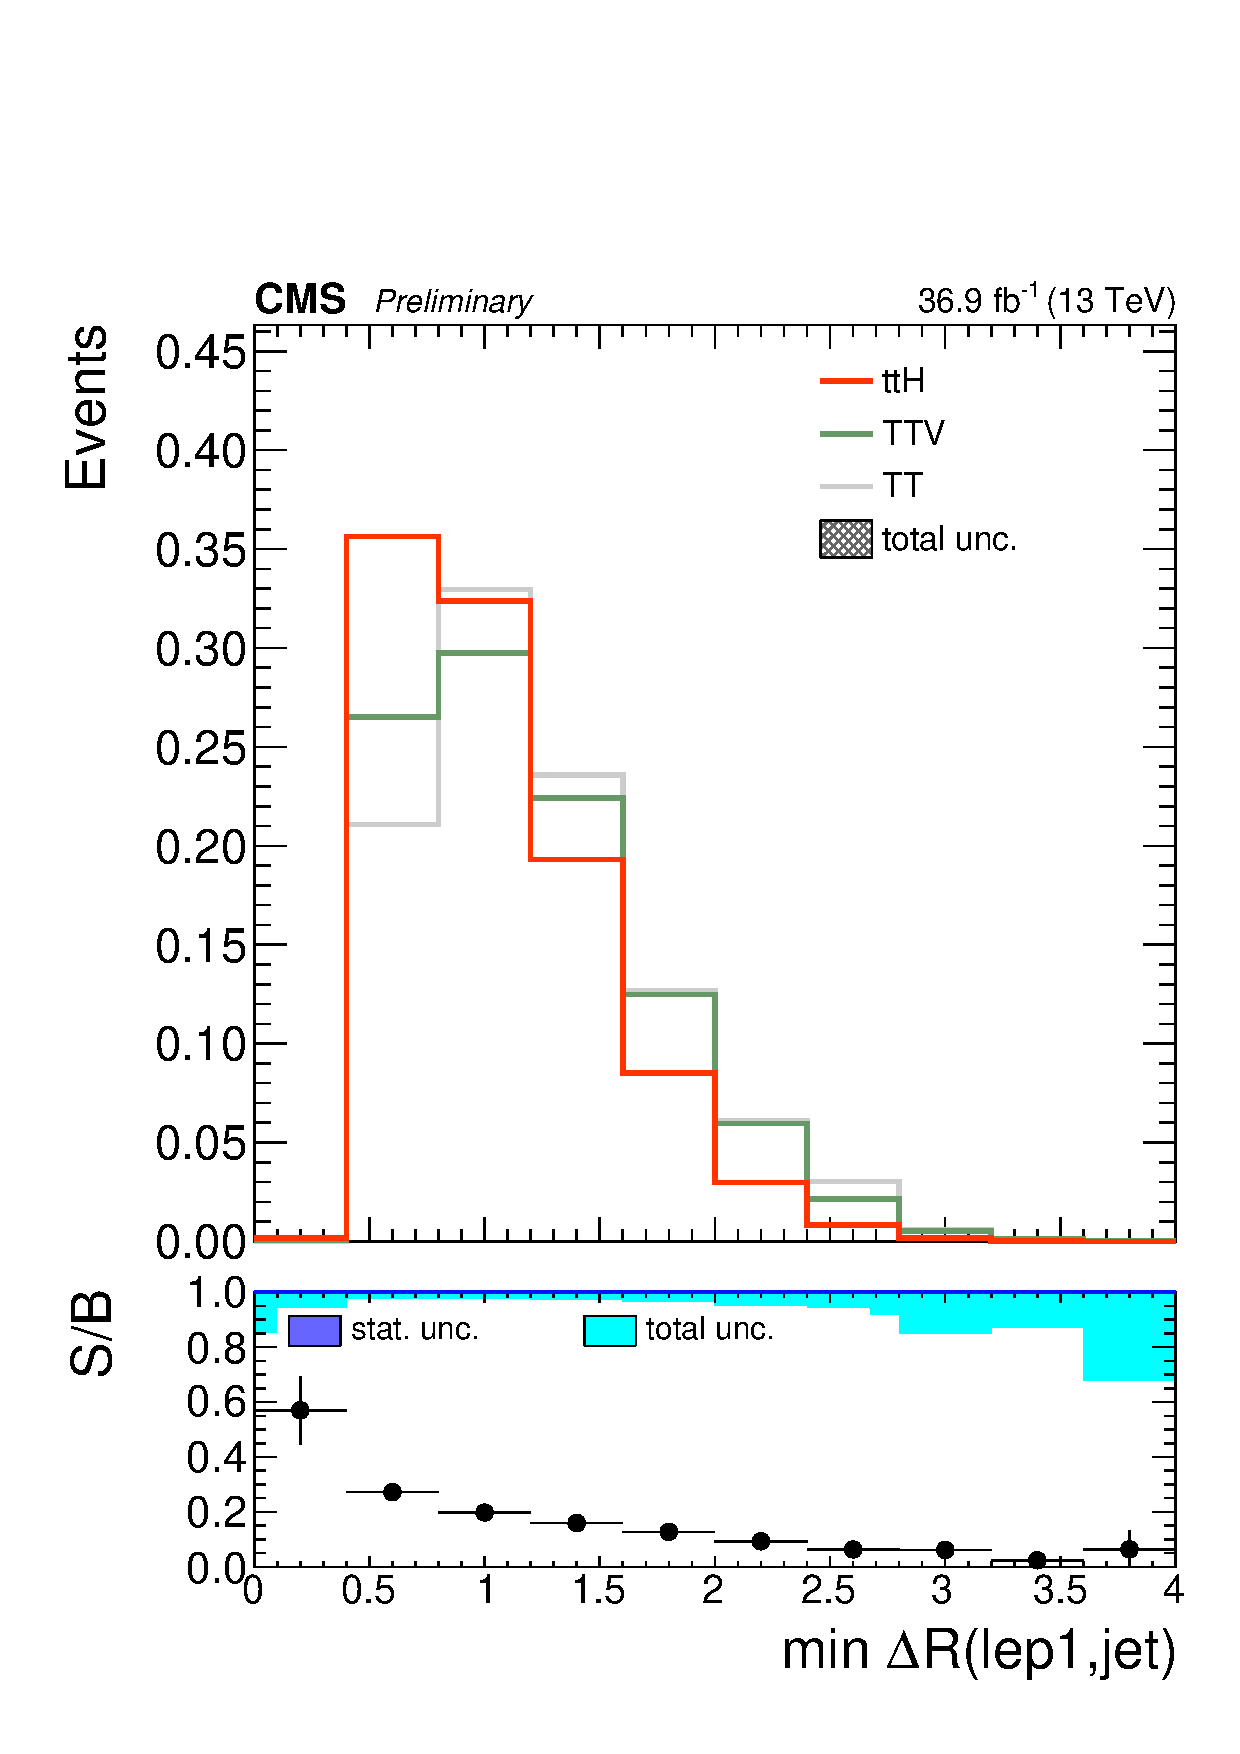
\includegraphics[width=0.3\textwidth]{ch9_figs/kinMVA_input_mindr_lep1_jet.pdf}
\caption[Signal extraction BDT input variables]{Normalized BDT input variable distributions for \tth and largest backgrounds}
\label{fig:inputs1}
\end{figure}

\begin{figure}[htp]
\centering
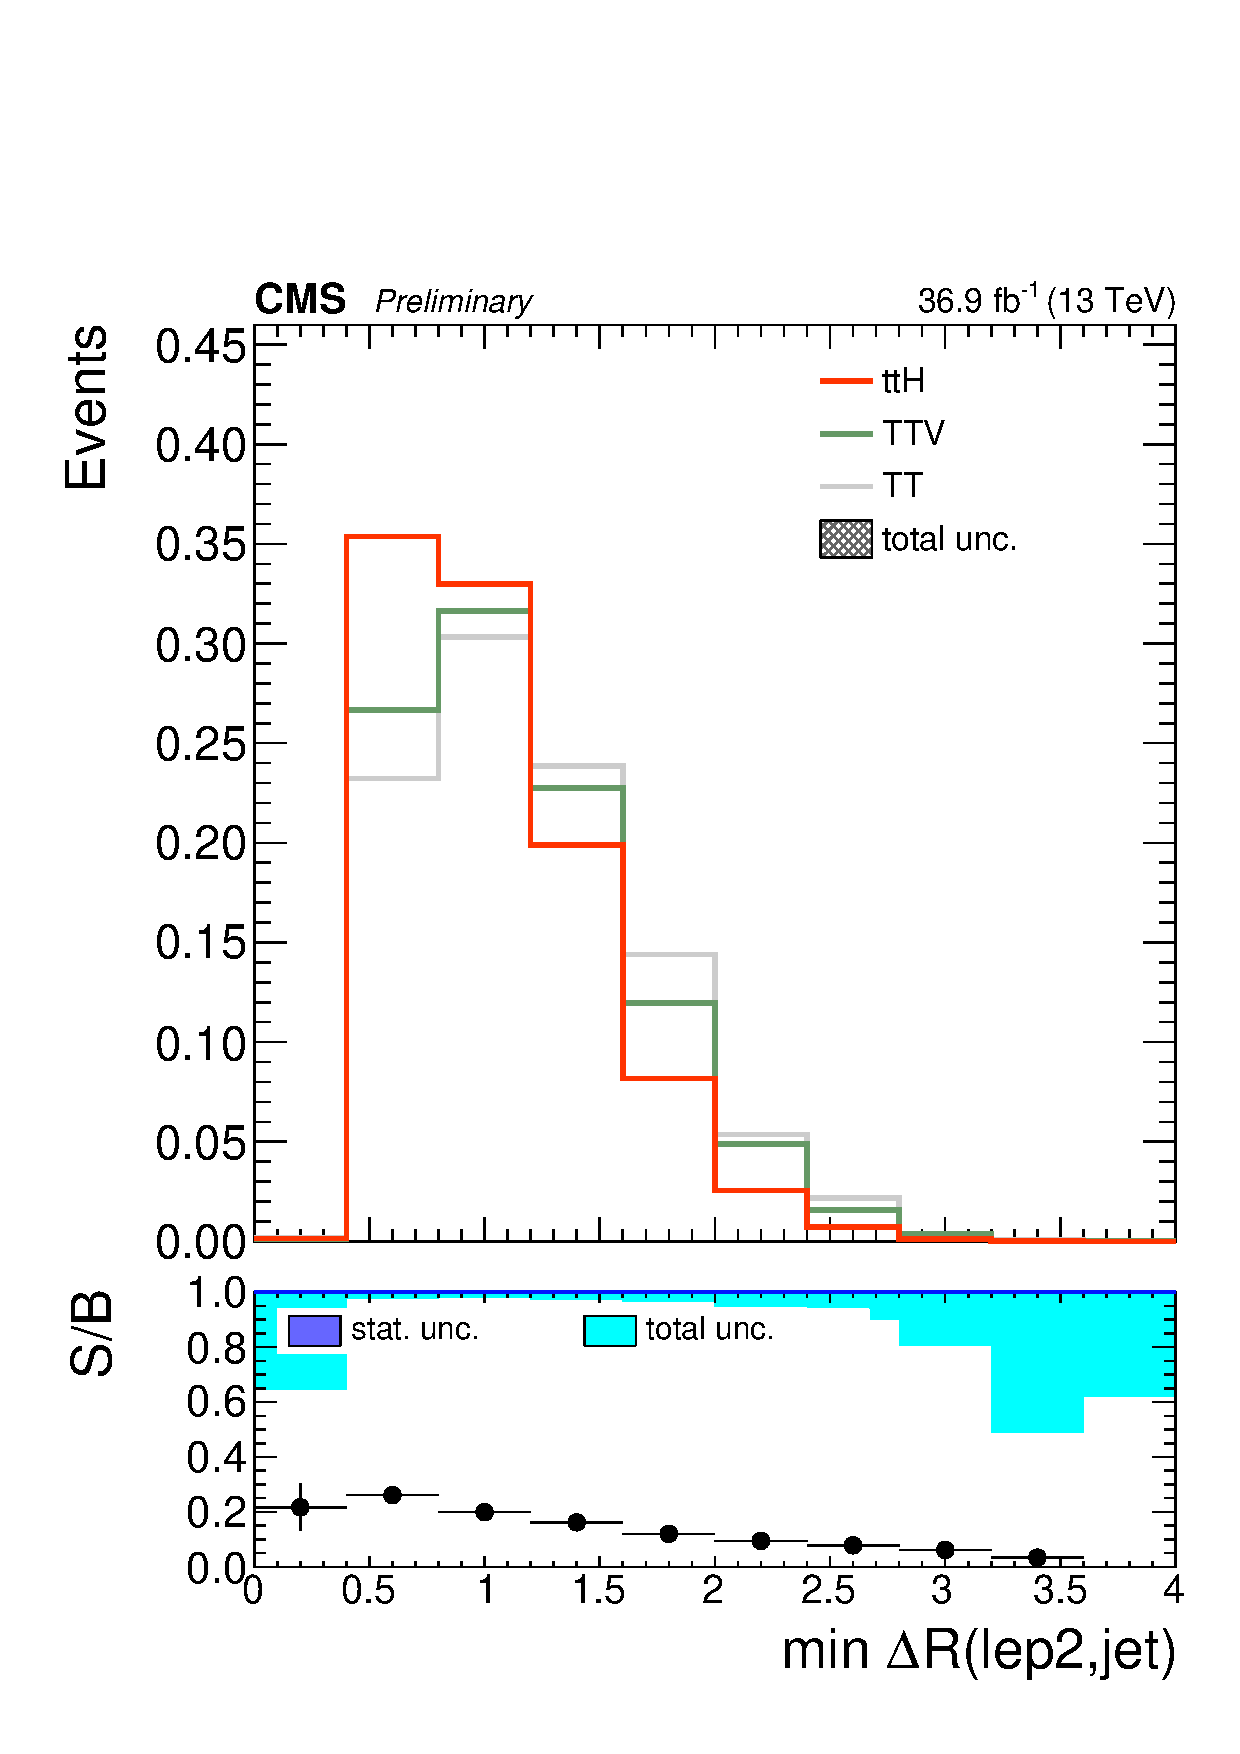
\includegraphics[width=0.3\textwidth]{ch9_figs/kinMVA_input_mindr_lep2_jet.pdf}
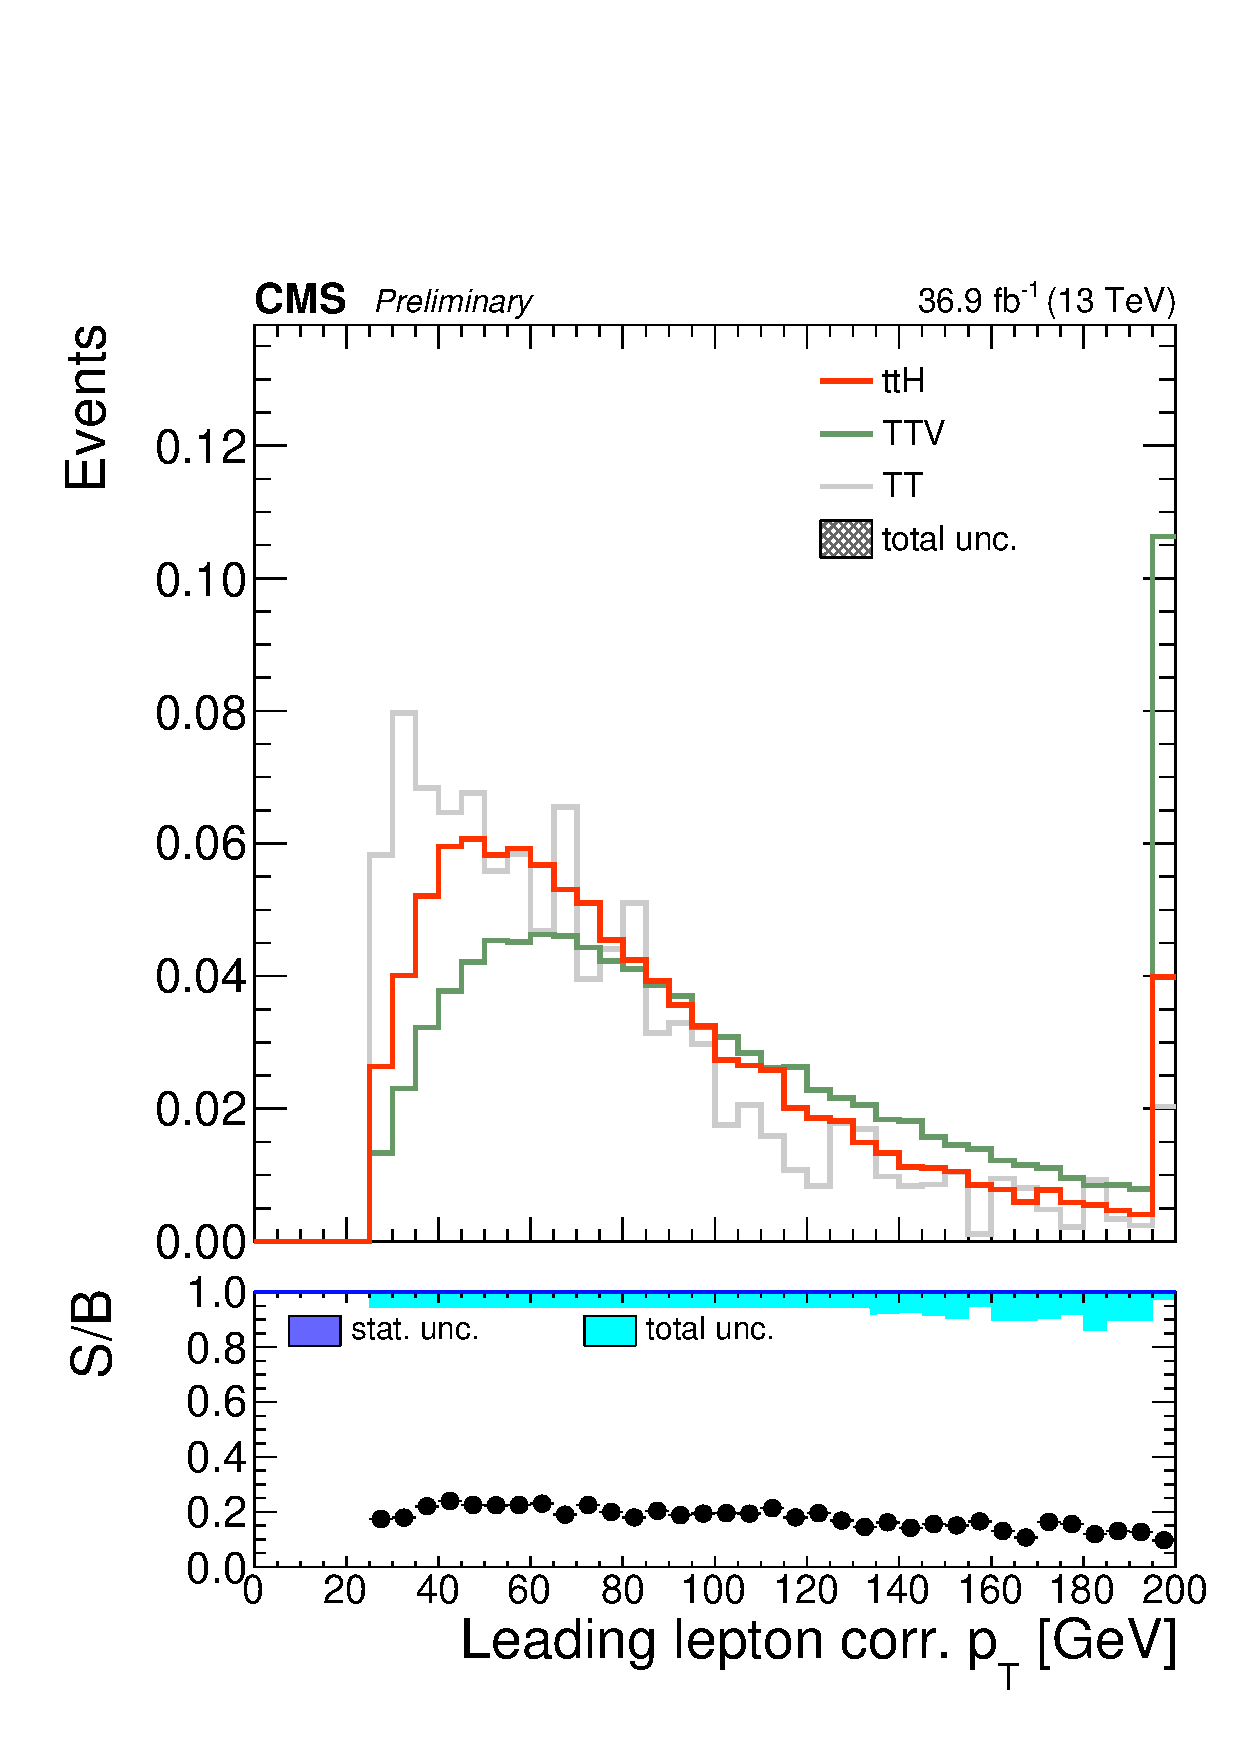
\includegraphics[width=0.3\textwidth]{ch9_figs/kinMVA_input_LepGood0_conePt.pdf}
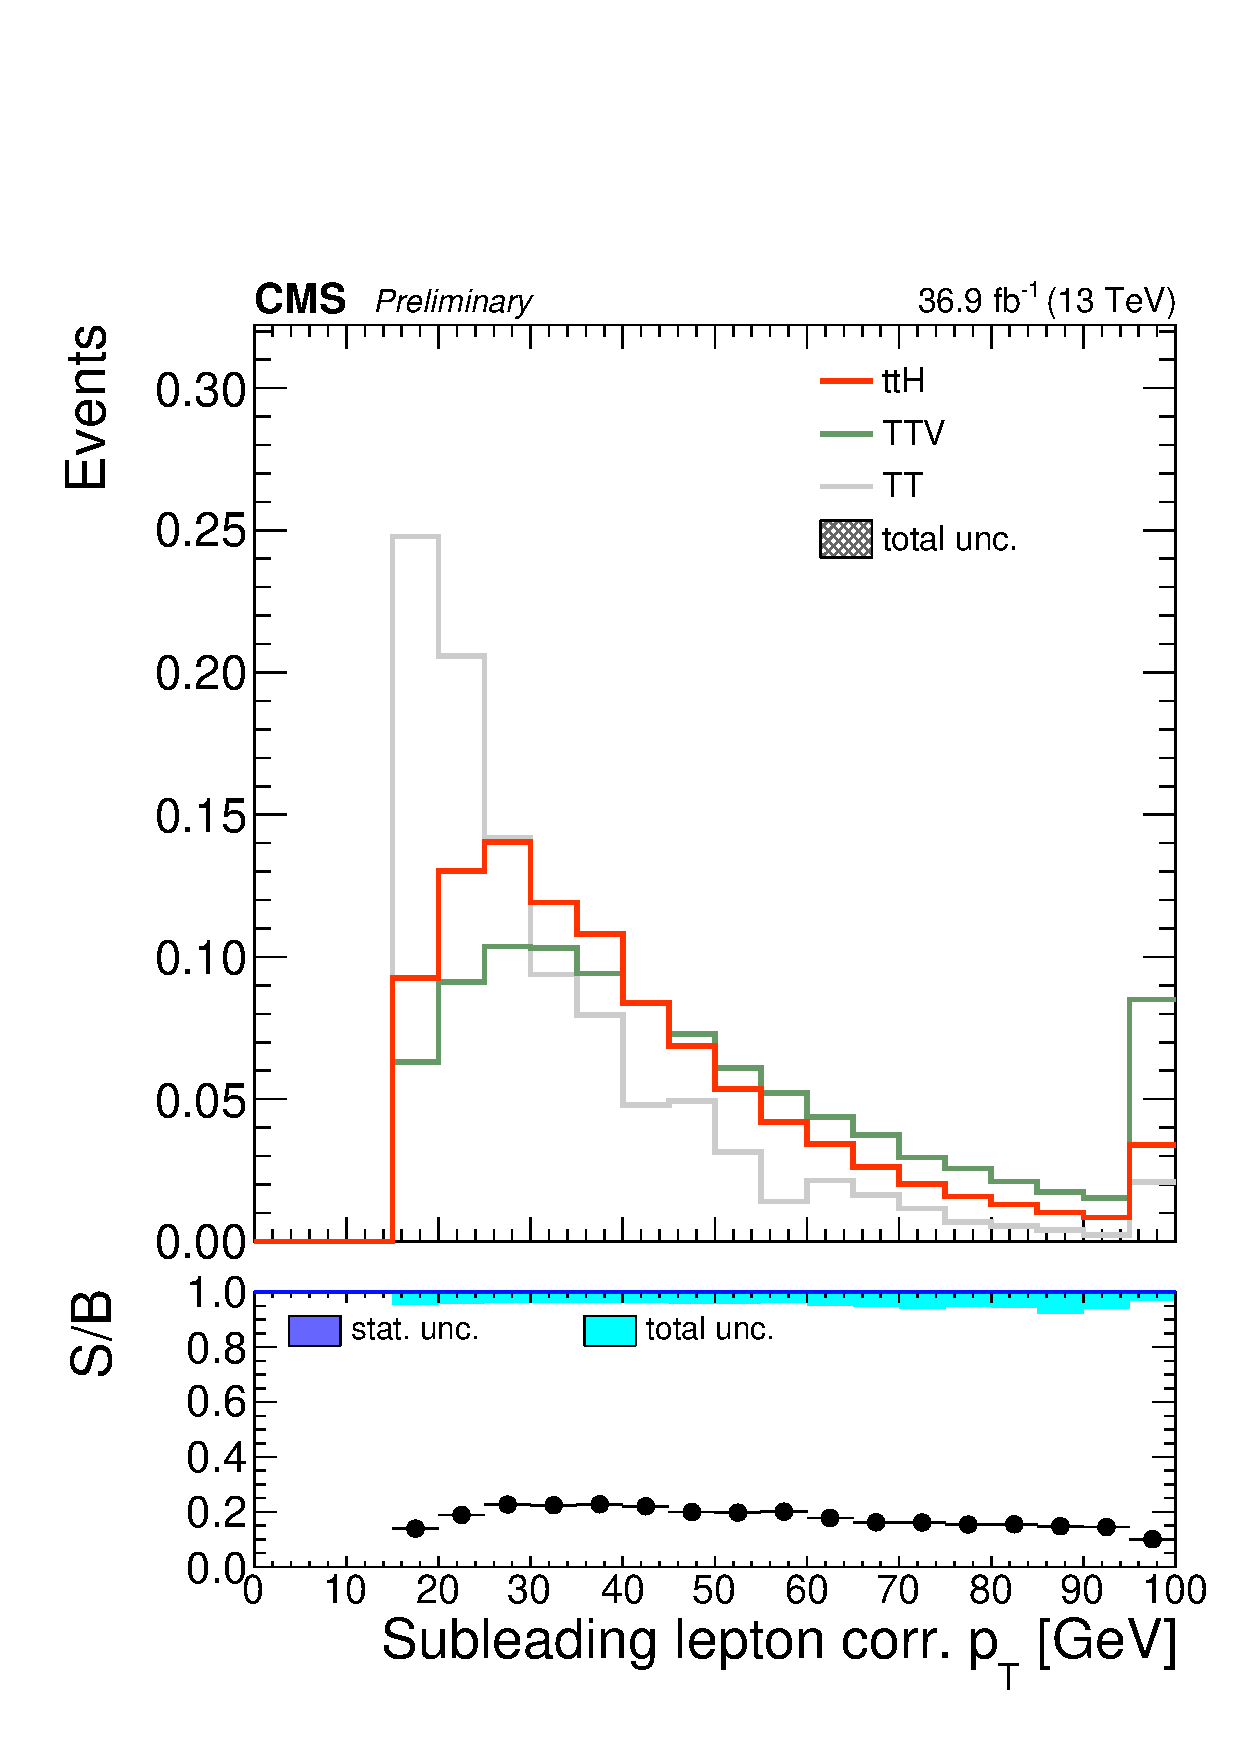
\includegraphics[width=0.3\textwidth]{ch9_figs/kinMVA_input_LepGood1_conePt.pdf}
\caption[Signal extraction BDT input variables]{Normalized BDT input variable distributions for signal and largest backgrounds}
\label{fig:inputs2}
\end{figure}

\begin{figure}[htp]
\centering
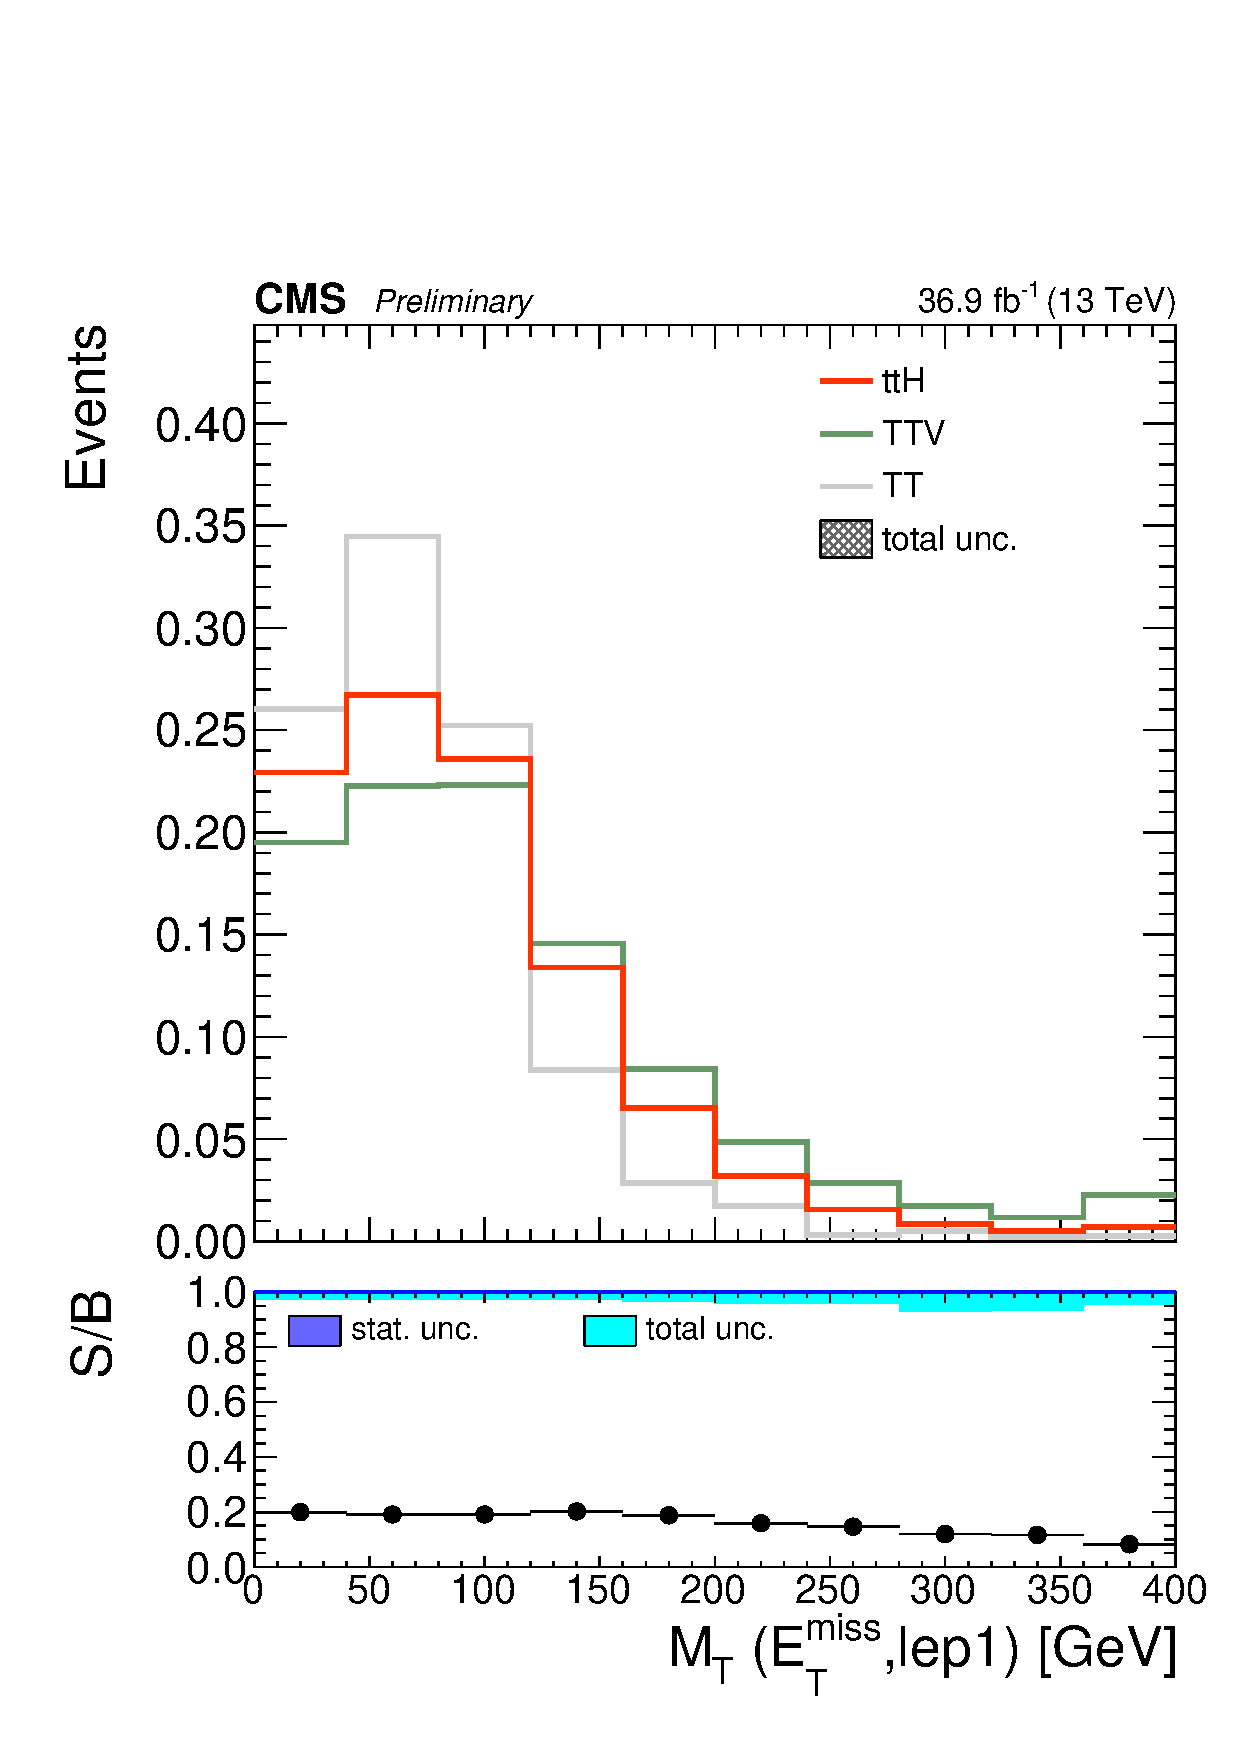
\includegraphics[width=0.3\textwidth]{ch9_figs/kinMVA_input_MT_met_lep1.pdf}
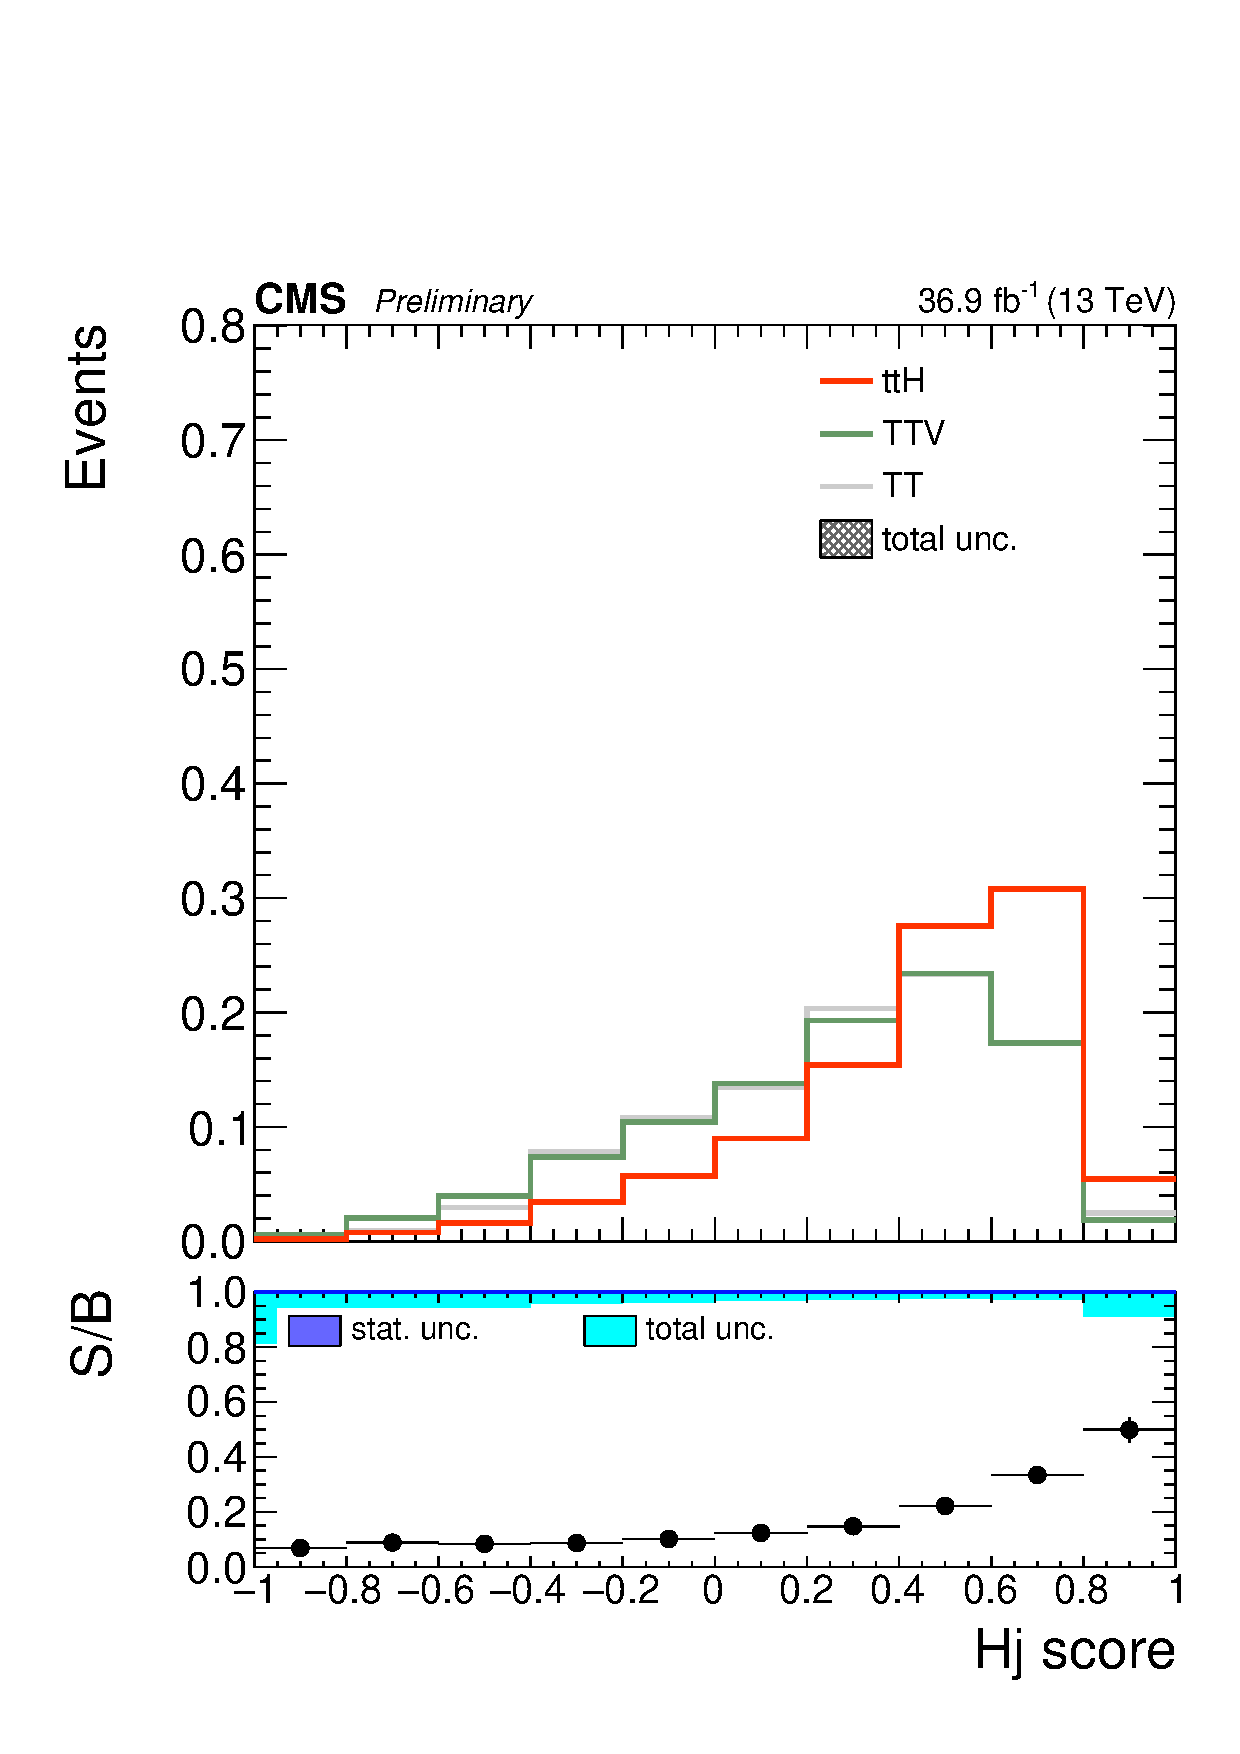
\includegraphics[width=0.3\textwidth]{ch9_figs/kinMVA_input_BDTv8_eventReco_Hj_score.pdf}
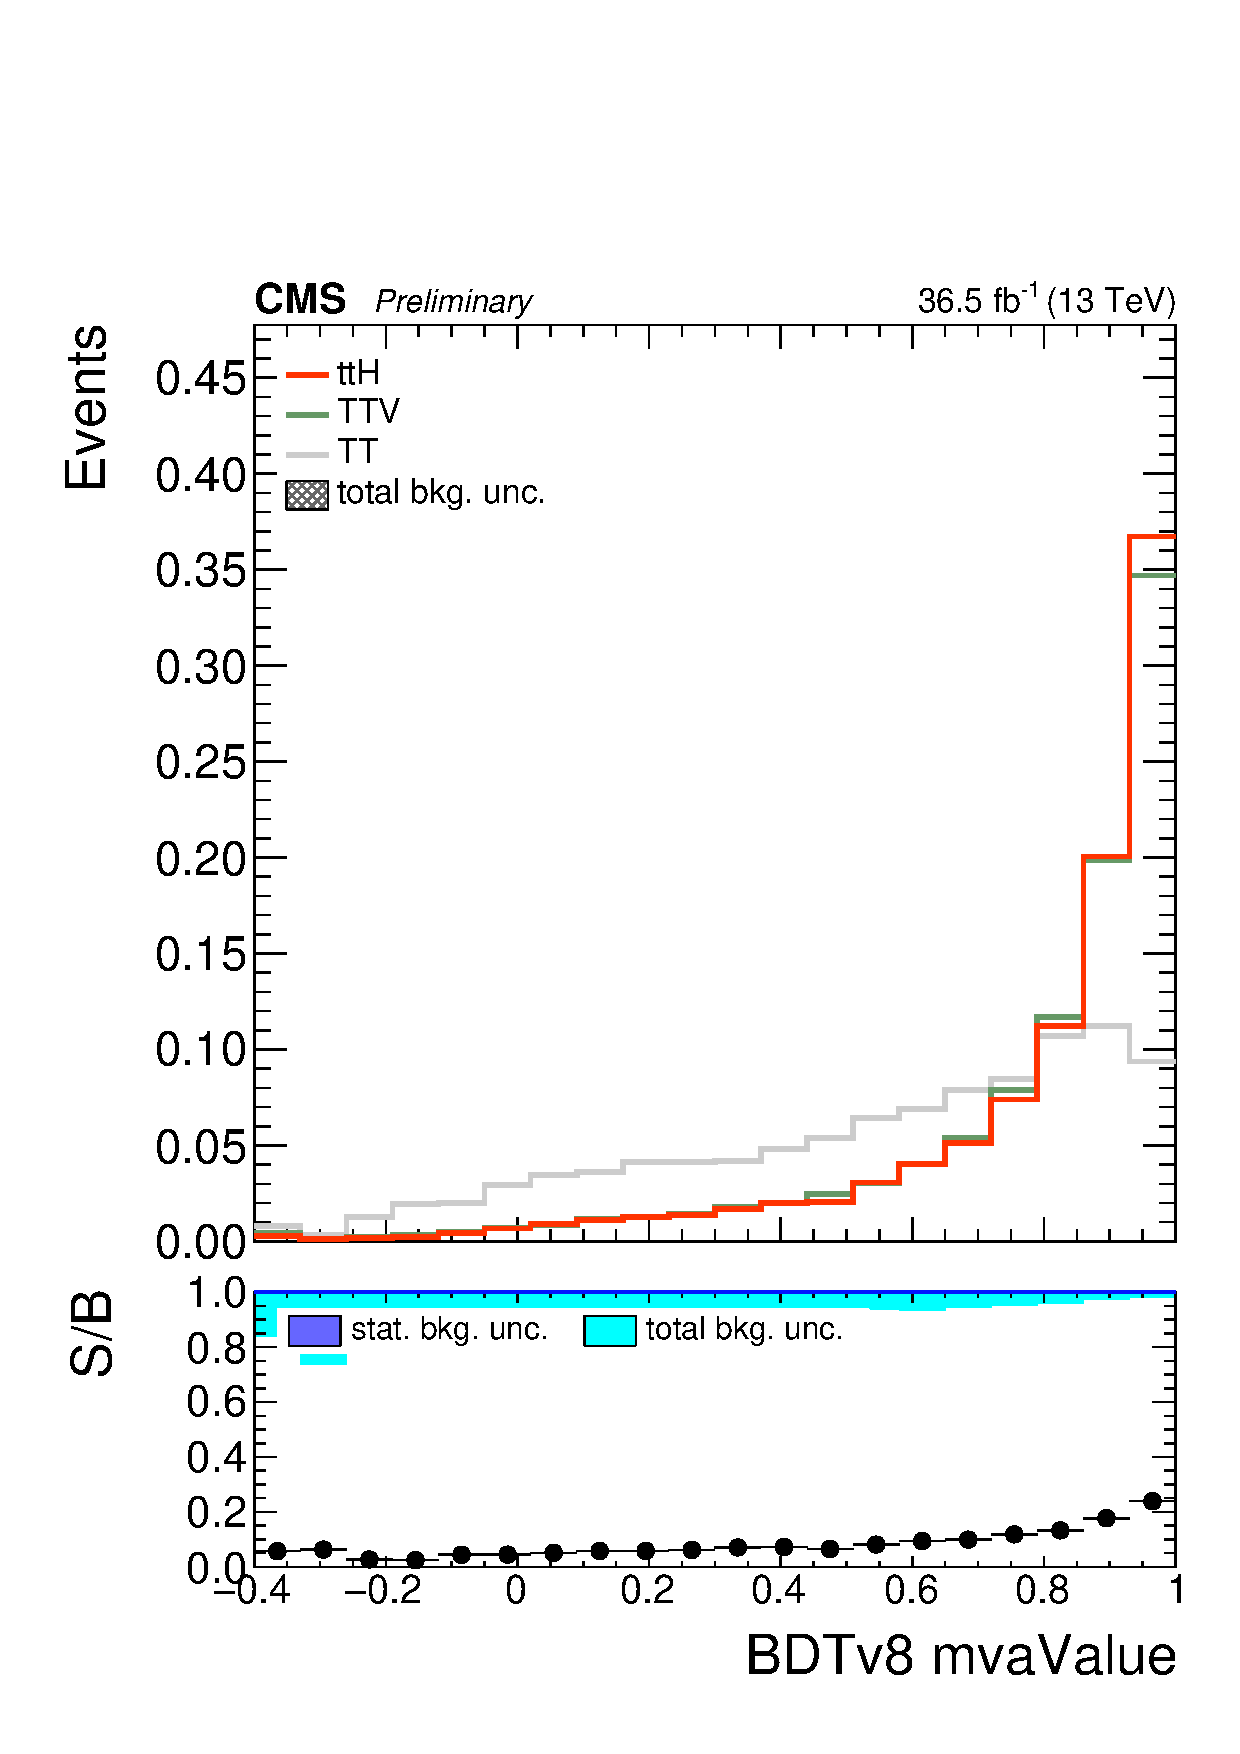
\includegraphics[width=0.3\textwidth]{ch9_figs/kinMVA_input_BDTv8_eventReco_mvaValue.pdf}
\caption[Signal extraction BDT input variables]{Normalized BDT input variable distributions for signal and largest backgrounds}
\label{fig:inputs2.5}
\end{figure}

\begin{figure}[htp]
\centering
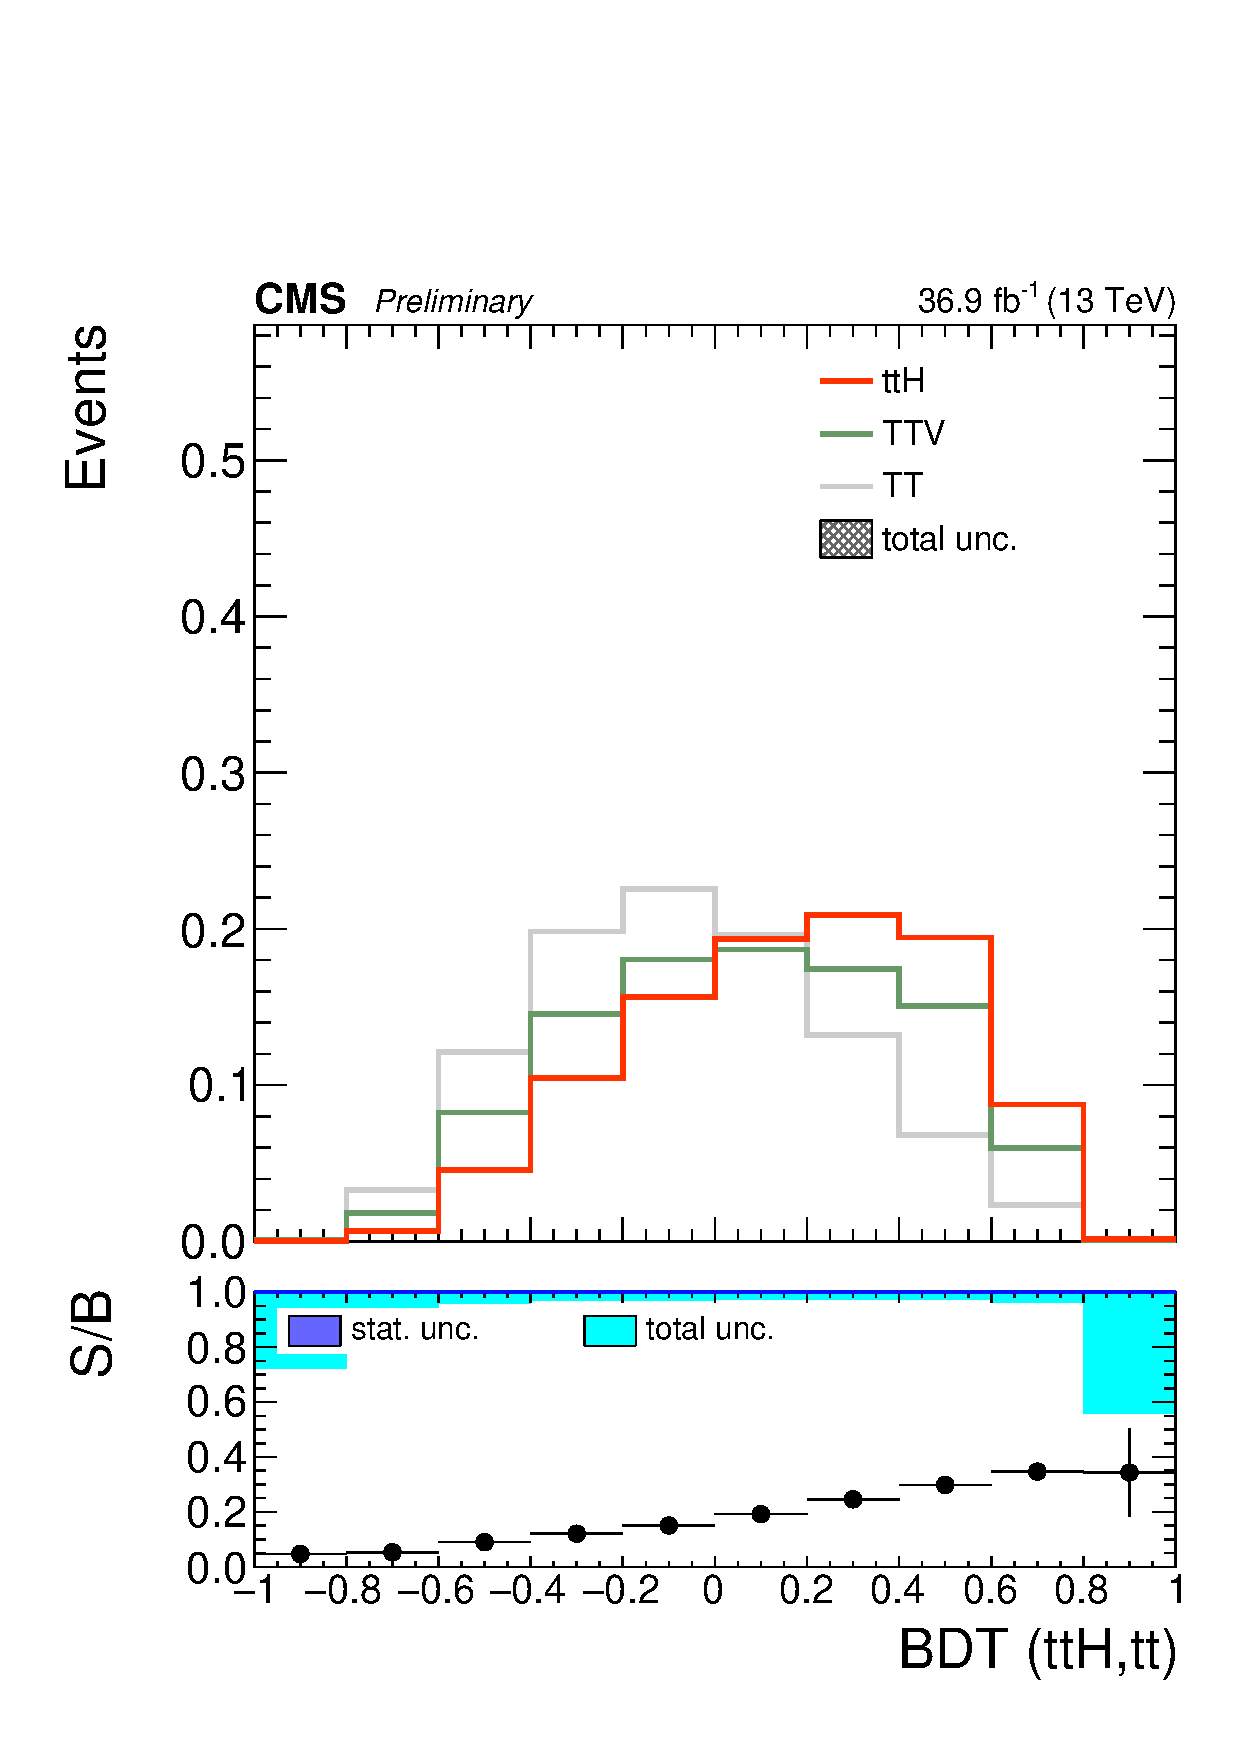
\includegraphics[width=0.49\textwidth]{ch9_figs/kinMVA_2lss_ttbar.pdf}
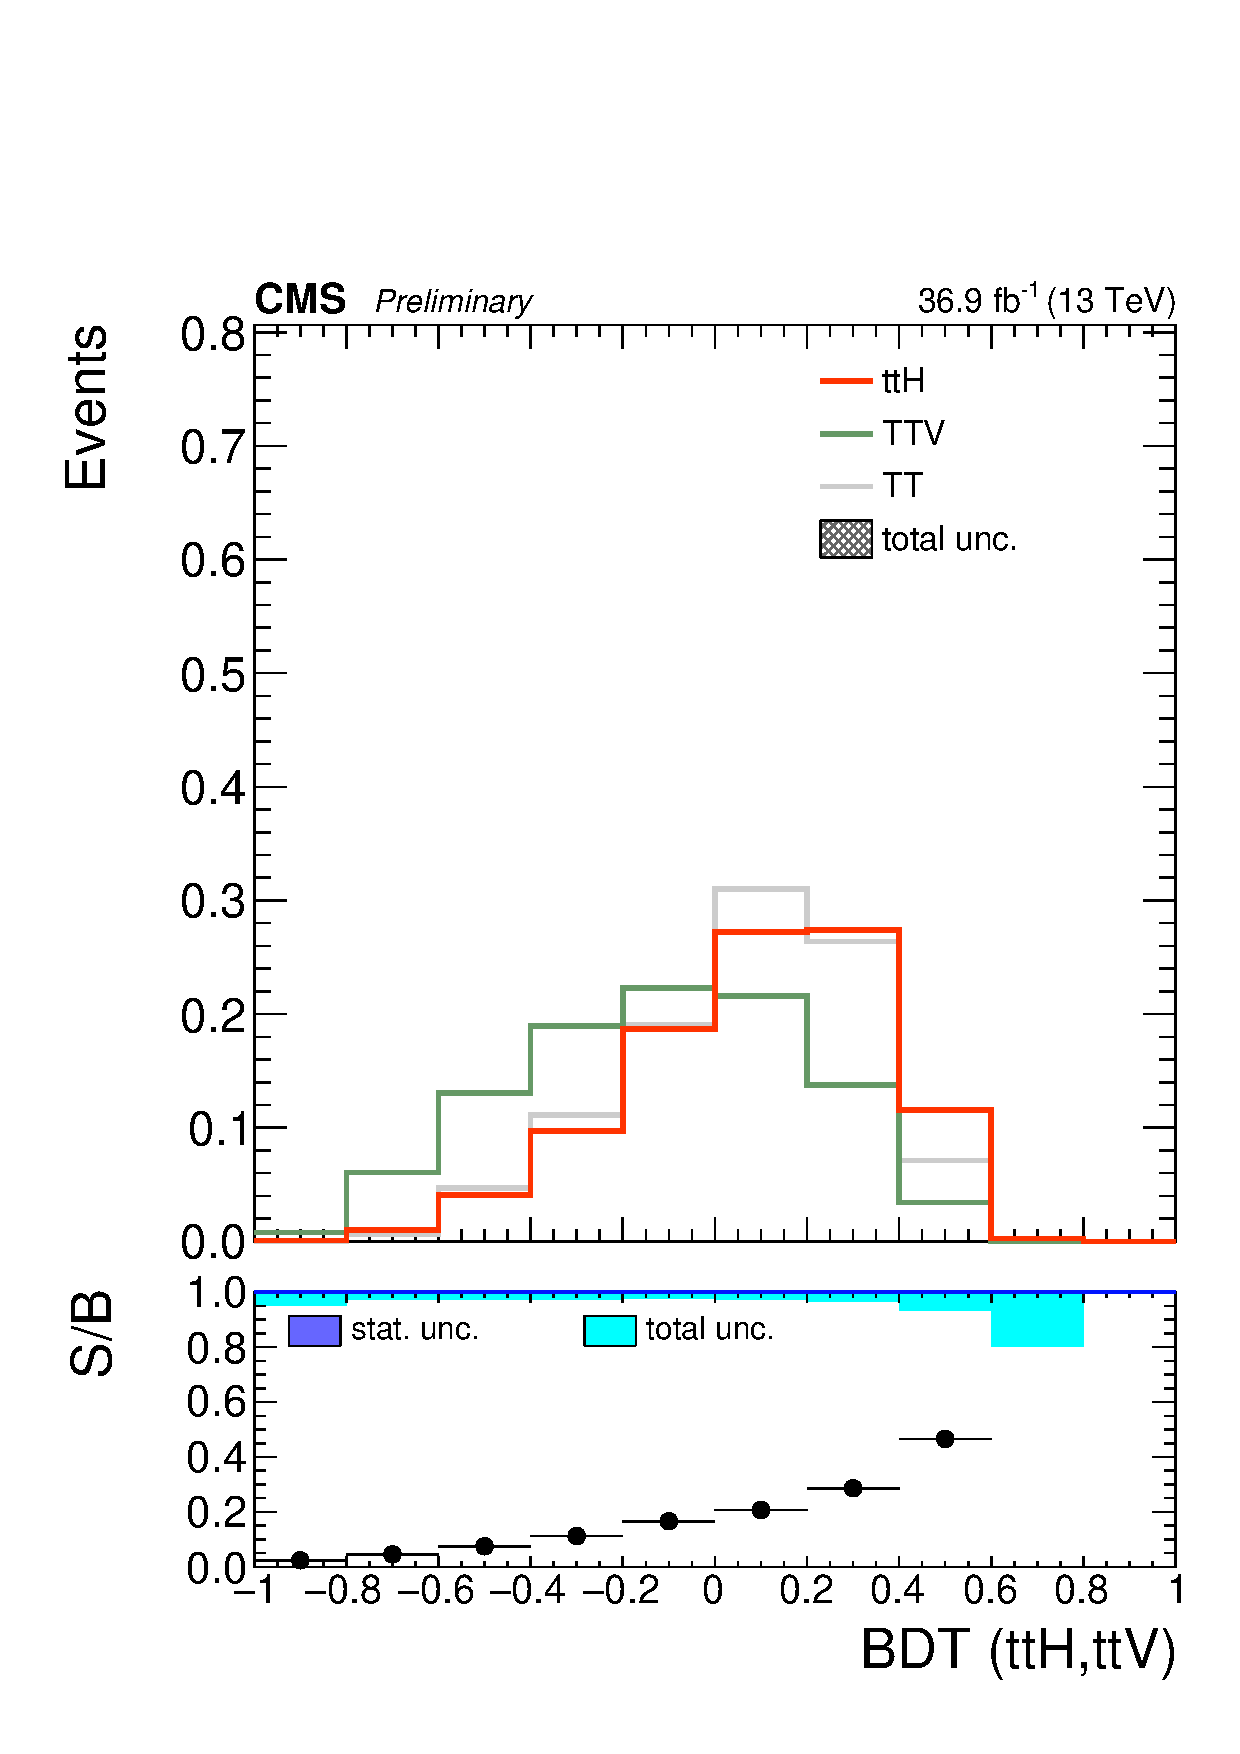
\includegraphics[width=0.49\textwidth]{ch9_figs/kinMVA_2lss_ttV.pdf}\\
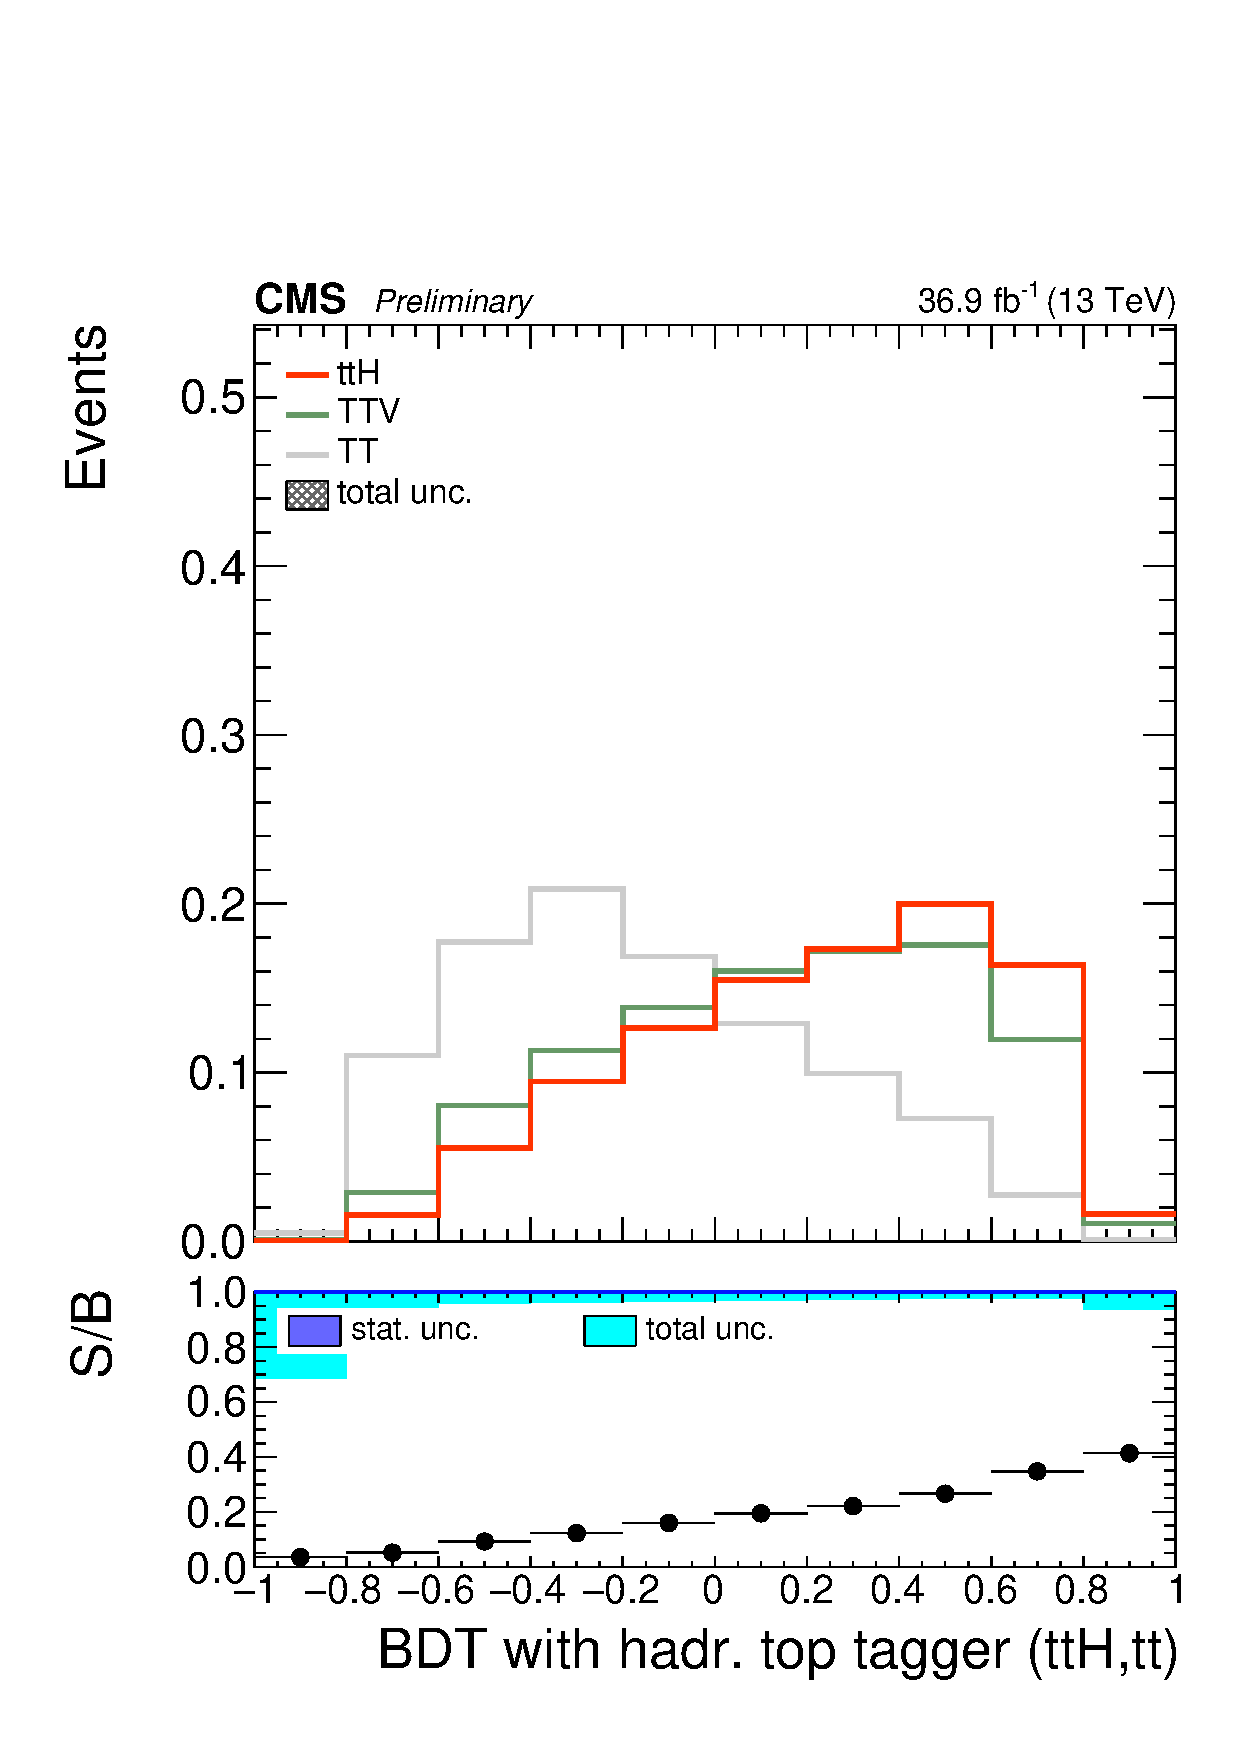
\includegraphics[width=0.49\textwidth]{ch9_figs/kinMVA_2lss_ttbar_withBDTv8.pdf}
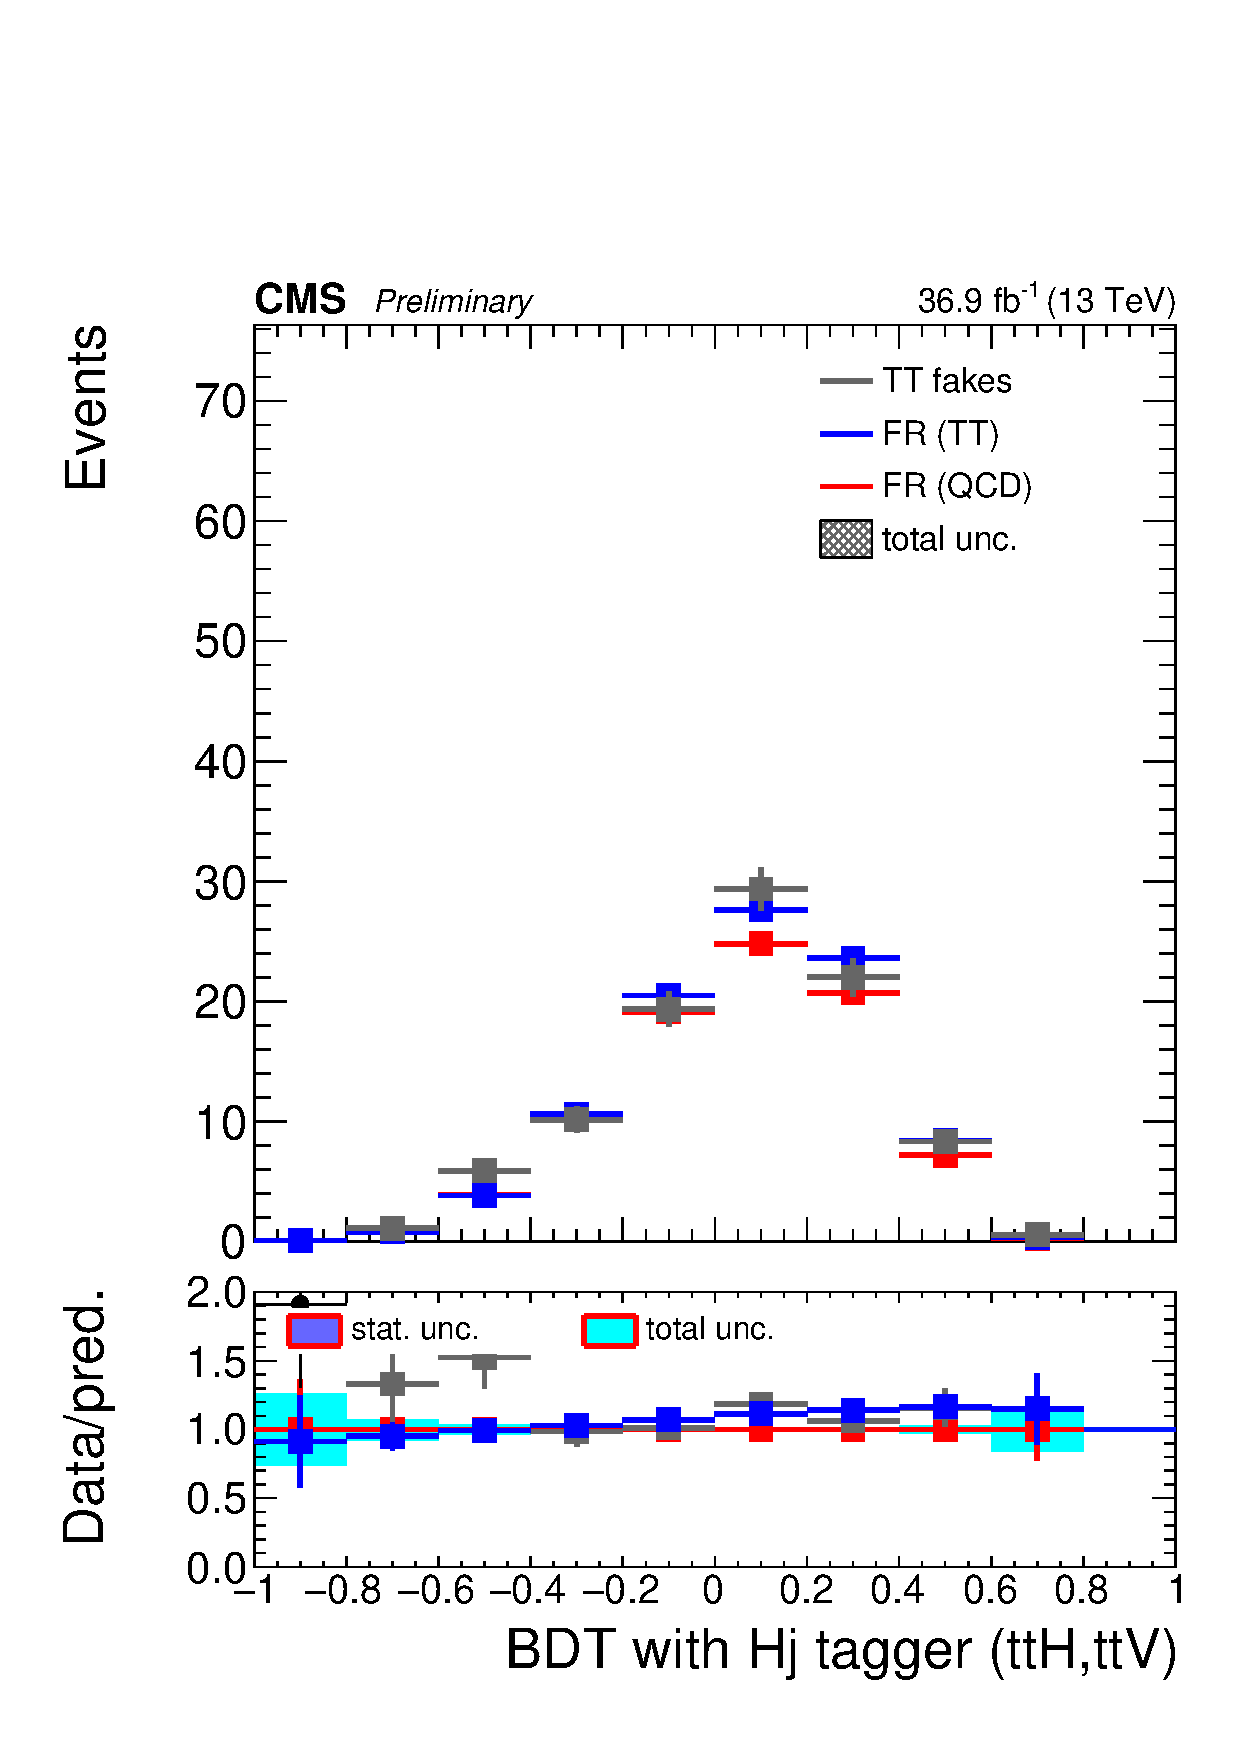
\includegraphics[width=0.49\textwidth]{ch9_figs/kinMVA_2lss_ttV_withHj.pdf}
\caption[BDT output scores with and without reconstruction inputs]{The BDT output scores without the reconstruction inputs (top) and with (bottom).}
\label{fig:inputs3}
\end{figure}

\subsection{Hadronic Top Reconstruction}
The hadronic top reconstruction input variable for the 2D BDT is the BDT output score of a special BDT, known as the hadronic top BDT,
that aims to correctly match jets in each event with the final state particles assocaited with the hadronic top in a 
a $t\bar{t}H$ event. The hadronic top BDT is evaluatd on every unique set of 3 jets in each event, with the highest-scoring combination
being designed as the hadronic top part of the event. The hadronic top BDT score gauges the likelihood that a jet combination is
consistent with a hadronic top in a \tth event, offering discrmination power against events without hadronically decaying top quarks, such as
semi-leptonic \ttbar.

This hadronic top reconstruction targets the 2lss category, specifically where the Higgs decays
to $W$ bosons. In the 2lss category, this means that one lepton originates from the
top system, and the other from the Higgs. For the jets, one of the
$W$ bosons from the Higgs decays hadronically, and one of the top quarks decays
hadronically. In total, there are two b-jets (one from each top) and four light-flavor jets
from the hadronic $W$ decays originating from the Higgs and the hadronic top.
This specific decay is depicted by the diagram in Figure~\ref{fig:intro_feyn}, and is the most common \tth decay in the 2lss channel.

\subsubsection{Training}
The hadronic top BDT is trained using the $t\bar{t}H$ MC powheg
signal sample used in training the final discrimination BDTs described previously.

The signal for training is $t\bar{t}H$ MC events, where a matching was performed on the final state objects, ensuring
they originate from the \tth part of the event, and not from ISR/FSR or spurrious detector signals in the detector simulation. This process
is called gen-matching, because the objects are required to originate from the event generator itself, and not the detector simulation which
follows. These events must pass the same loosened training selection
described in Section~\ref{sec:2D_BDT}, with one important difference. In the selection used
here, the same-sign requirement on the leptons is dropped. This doubles the amount of events available
for training and the gen-matching requirement ensures the signal kinematics are left unaffected. 
The 2lss event selection requires at least four jets, which means the vast majority of signal
events used for training are only partially reconstructed since a full reconstruction
necessitates six matched jets. Because so few events can be fully reconstructed, we must
consider partial reconstructions for events that have fewer than six matched jets.
The strategy for this is to use ``null'' jets whose four-vectors are set to zero to
represent missing jets in the event. Finally we require the signal events to have two
correctly-matched selected leptons, and at least four correctly-matched selected jets.

The background consists of all jet and lepton permutations of incorrectly-matched
$t\bar{t}$ events. This means that in each background event, there must be at least one
object that is incorrectly matched. For example when considering the object-matching to the
leptonically decaying top quark, a background training event where the reco-level jet assigned
to the b-jet, is actually the b-jet at gen-level, the reco-level lepton must originate from some source
other than the W from the leptonically decaying top. In this way, a single \ttbar MC
background event is used multiple times, once for each distinct permutation of 6 objects, in the training.
This technique produces more background training events than necessary given the limited (in comparison)
signal training statistics.

For the background, the null jets are added according to the
jet multiiplicity. For events with seven or fewer selected jets, three null jets are
added, for events with eight selected jets, two null jets are added, and one null jet
is added for events with greater than eight selected jets. The motiviation for this recipe
comes from a study of \tth events in the signal region comparing the number of reco jets that are
gen-matched to the \tth process, with the jet multiplicity in the event. The results of this study are
in Figure~\ref{fig:jet_matching}. 

\begin{figure}[htp]
\centering
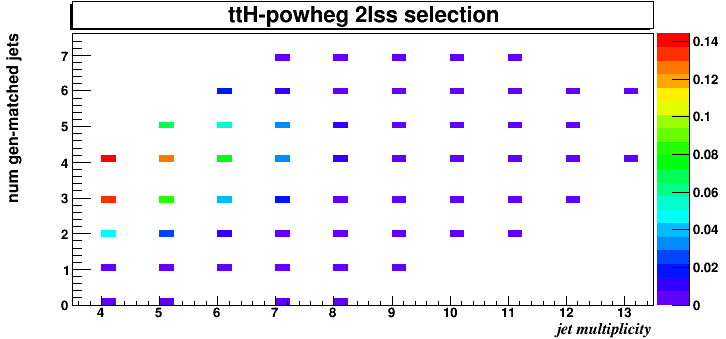
\includegraphics[width=0.49\textwidth]{ch9_figs/jet_matching.png}
\caption[Comparison of gen-matched jet multiplicity to jet multiplicity in signal events]{ Normalized histogram of gen-matched jet multiplicity vs jet multiplicity in \tth MC in the signal region.}
\label{fig:jet_matching}
\end{figure}

To reduce the computation time and improve performance,
several cuts are applied at each permutation to remove unlikely reconstructions.
These cuts include applying the b-tag requirement on the two jets being considered
as b-jets described earlier, requiring that no
reconstructed $W$ have a mass greater than 120 GeV, requiring the leptonic top mass
be less than 180 GeV, and requiring 
the hadronic top mass be less than 220 GeV. Additionally, we ignore permutations
arising from swapping two light flavor jets from the same $W$ boson, as the reconstruction is
identical.
An additional measure is taken to reduce iterations over each permutation, in the training step and for background only,
which samples randomly from the available permutations in each event before the phyics-motivated cut is applied.
For each of the 8 objects, the permutation for that object skipped randomly 3 out of 10 times. For 8 objects,
this means that $0.7^{8} \approx 0.06$ or just 6$\%$ of the permutations for a given event are considered. After factoring
in the permutations skipped due to physics cuts, this number is even smaller. It was found that the increase in statistics
from removing these random cuts offers negligible improvement in performance while drastically increasing the CPU time used
during training.

The BDT uses eight input variables, consisting of:
\begin{itemize}
\item The CSVv2 score of the b-jet assigned to the hadronic top
\item The CSVv2 score of the b-jet assigned to the leptonic top
\item The transverse momentum of the reconstructed hadronic top
\item The mass of the reconstructed hadronic top
\item The mass of the $W$ boson from the hadronic top
\item The transverse momentum ratio of the lepton from the Higgs to the lepton from the leptonic top
\item The solid angle between the lepton from the leptonic top and the b-jet from the hadronic top
\item The solid angle between the lepton from the leptonic top and the b-jet from the leptonic top
\item The solid angle between the lepton from the Higgs and the b-jet from the leptonic top
\end{itemize}

\subsubsection{Evaluation}
The hadronic top BDT is evaluated by iterating over all possible lepton and jet
permutations, and selecting the highest scoring permutation as the reconstruction for
each event. For this evaluation, the null jet prescription and permutation
cuts used are identical to the background training.
The reconstruction is designed identify events that have a hadronic top present and
discriminates against the semi-leptonic $t\bar{t}$ background. The addition of the 
reconstruction BDT output as an input to the BDT targeting the $t\bar{t}$ background,
improves the performance by 10$\%$ by comparing ROC integrals\footnote{Receiver Operator Characteristic (ROC), curves quantify the separation of two distributions, such as signal and background,
of a variable, such as BDT output, at all values of that variable. Every point on a ROC curve corresponds to a specific value of the variable. At each value of the variable, the fraction of one
distribution that falls above that value, and the fraction of the other distribution that falls below that value form an (x,y) point on the ROC curve. The curve is then generated by scanning over
the range of the variable which contains both distributions, adding a point for each value of the variable and connecting the points with a curve. As the separation of the two distributions increases,
the larger the area under the ROC curve. It is this property that makes ROC curves a useful metric for evaluating BDT output performance.}
when evaluated on $t\bar{t}$ MC and compared to the
equivalent BDT in the 2016 \tth ICHEP analysis~\cite{CMS-AN-16-022} that did not use this
as an input. These performance ROC curves are below in Figure~\ref{fig:hadtop_performance}.

\begin{figure}[htb]
 \centering
   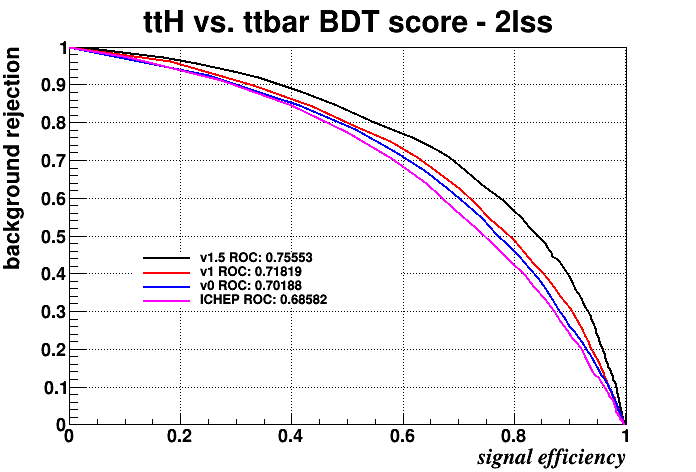
\includegraphics[width=0.6\textwidth]{ch9_figs/improvement_roc.png}
   \caption[ROC curves of $t\bar{t}$ BDT with and without hadronic top reconstruction input]{The ROC curves of the BDT targeting the $t\bar{t}$ background compared without 
   hadronic top reconstruction input (pink) to the version used in this analysis (black). The other curves represent incremental improvements to the hadronic top BDT. The signal
   and background on the x and y axes are \tth and \ttbar MC respectively. The improvement based on ROC integral by adding the hadronic top reconstruction score is 10$\%$.}
  \label{fig:hadtop_performance}
\end{figure}

\subsection{Higgs Jet Tagging}
The Higgs Jet (HJ) tagger is a BDT aimed specifically at identifying hadronic jets originating from the W bosons in \tth, H$\rightarrow$WW decays consistent
with the \tth diagram in Figure~\ref{fig:intro_feyn}. This decay topology is the most common of all \tth decays in the $2lss$ channel. This final state
consists of 2 b-quark jets, 4 hadronic (light flavor) jets, 2 same-sign leptons, and missing energy due to neutrinos. The signal region selection described
in Chapter~\ref{chap:event_selection} does not require all of these objects to be present, as some or many are often out of the acceptance. This means that
the jets from the Higgs decay could be missing entirely from the event.

The HJ tagger addresses both the complicated jet combinatorics associated with this final state, but also the reality that not all jets originating
from the Higgs are selected. The HJ tagger is an object-level discriminator that exploits jet kinematics and identification variables to estimate the likelihood
of a jet originating from the Higgs. The HJ tagger calculates scores for every jet in each event, selecting
the highest score as the output. To boost performance and simplify the combinatorics associated with tagging, the hadronic top tagger is first run,
and the jets selected as being assocaited with the hadronic top are removed from further consideration for the HJ tagger.
The HJ tagger is primarily aimed at selected jets from W decays (from the Higgs) and is used as a discriminating varible against both the \ttw and \ttz backgrounds.
Both of these
backgrounds are very likely to contain most or all of the hadronic top decay products, namely a b-tagged jet and two light flavor jets. The two light flavor jets from
the W in the hadronic top decay look kinematically similar to the targeted jets from the W from the Higgs, creating a potential for Higgs jet mis-tagging. This is
especially true when the b-jet is missing. The hadronic top tagger attempts to identify these jets and they are removed from consideration for the HJ tagger.

The HJ tagger is trained on \tth and \ttv MC. The signal training events require the objects passing the selection to be matched to a generator-level parton
originating from the H$\rightarrow$WW$\rightarrow l\nu~l\nu$ process. The background selection requires \ttv events in the signal region.  
The input variables include:
\begin{itemize}
\item the minimum angular separation between the jet and one of the two leptons
\item the maximum angular separation between the jet and one of the two leptons
\item the jet transverse momenta
\item the jet b-tag discriminator (CSVv2)
\item the jet quark-gluon discriminator (qgid)
\end{itemize}

\noindent The qgid varible is a BDT designed to discriminate jets originating from light flavor quarks from jets originating from gluons. The performance improvement due
to the HJ tagger input is seen in Figure~\ref{fig:hj_tagger}, and corresponds to approximately 4-5$\%$ increase in signal efficiency at the same background efficiency.
The data to MC comparison of both the hadronic top BDT and higgs tagger BDT ouputs are in Figure~\ref{fig:reco_bdt_stacks} below.

\begin{figure}[htp]
\centering
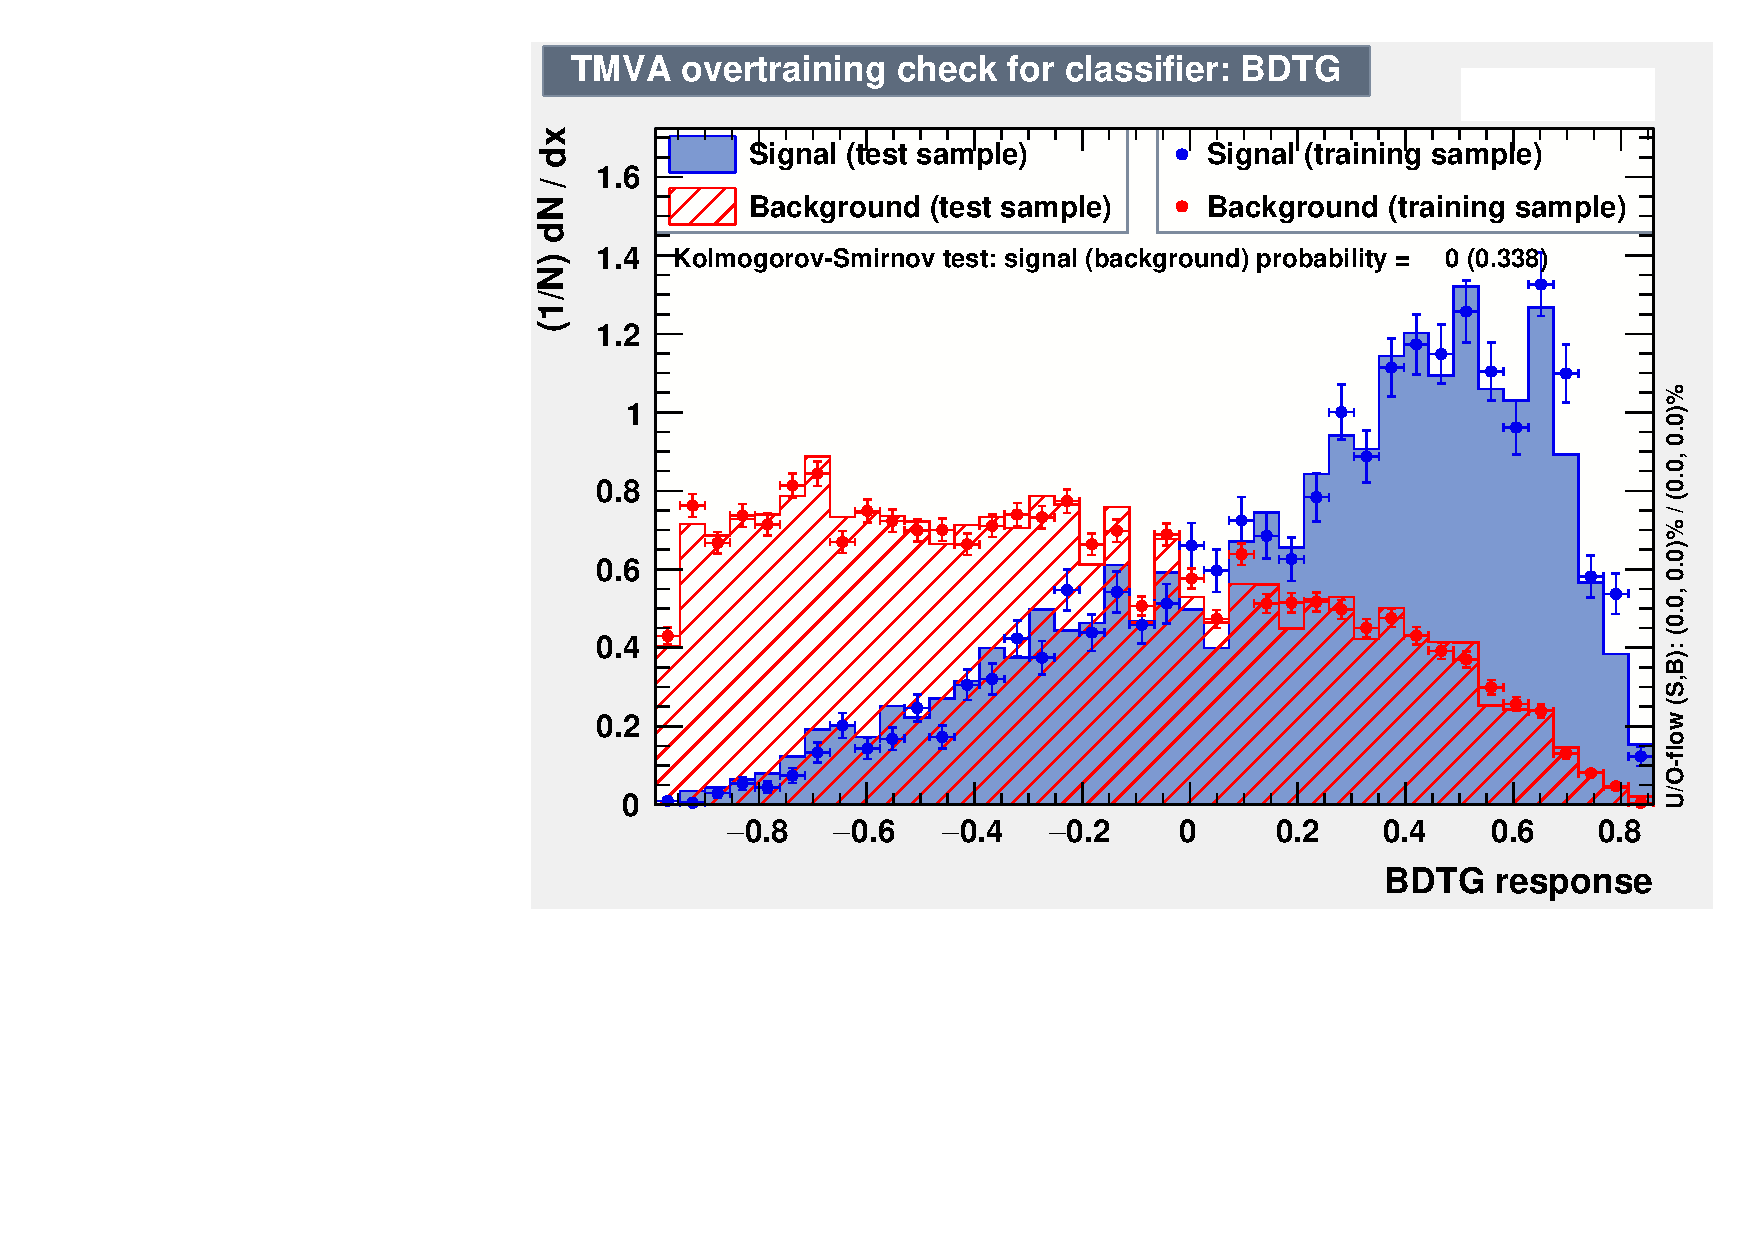
\includegraphics[width=0.49\textwidth]{ch9_figs/Jtagger_Ks.pdf}
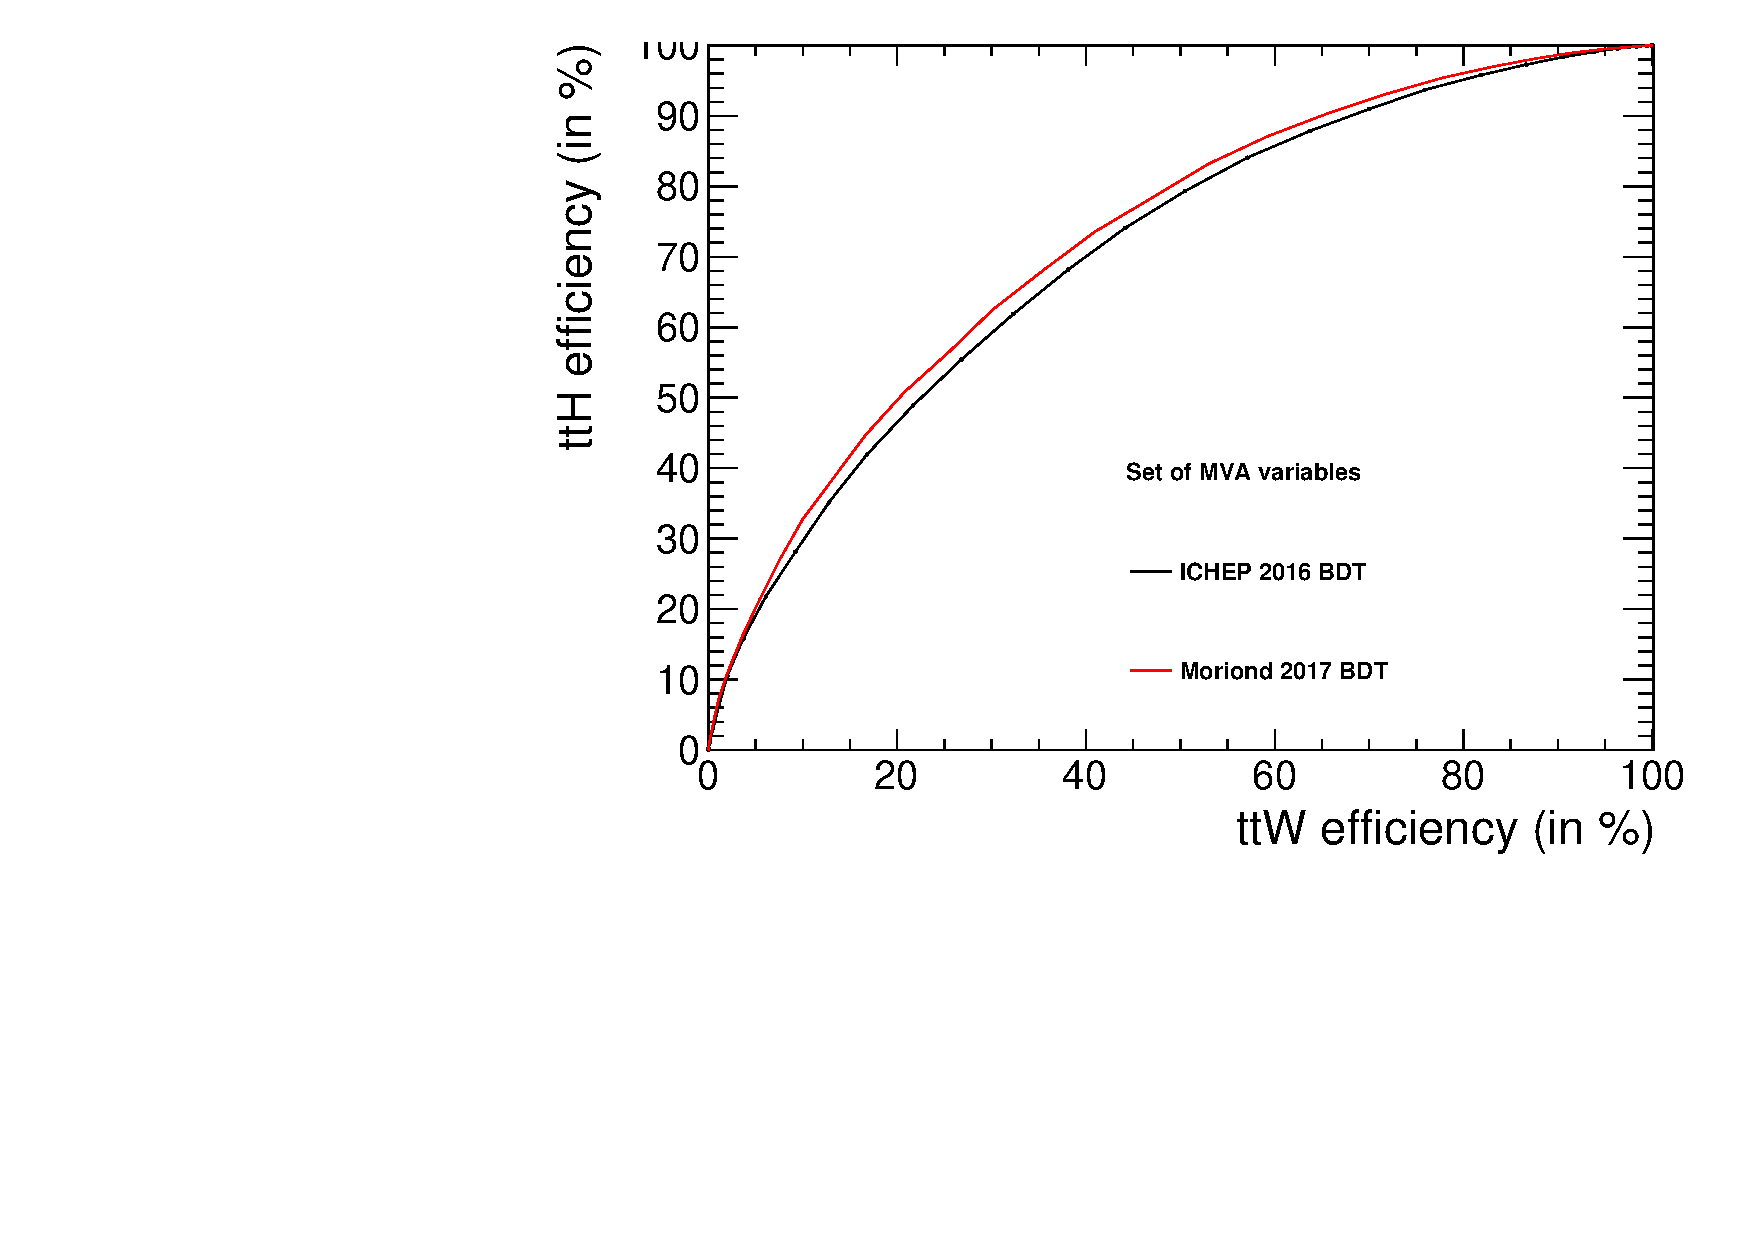
\includegraphics[width=0.49\textwidth]{ch9_figs/Roc_Comparison_18Feb.pdf}
\caption[Performance improvement from the HJ tagger and hadronic top removal]{Separation power of HJ output on the training samples (right) and performance improvements with respect to the 2016 version of this analysis obtained with the HJ
tagger input with hadronic top removal (left). Note the difference in axes with respect to the ROC curve for the hadronic top BDT.}
\label{fig:hj_tagger}
\end{figure}

\begin{figure}[htp]
\centering
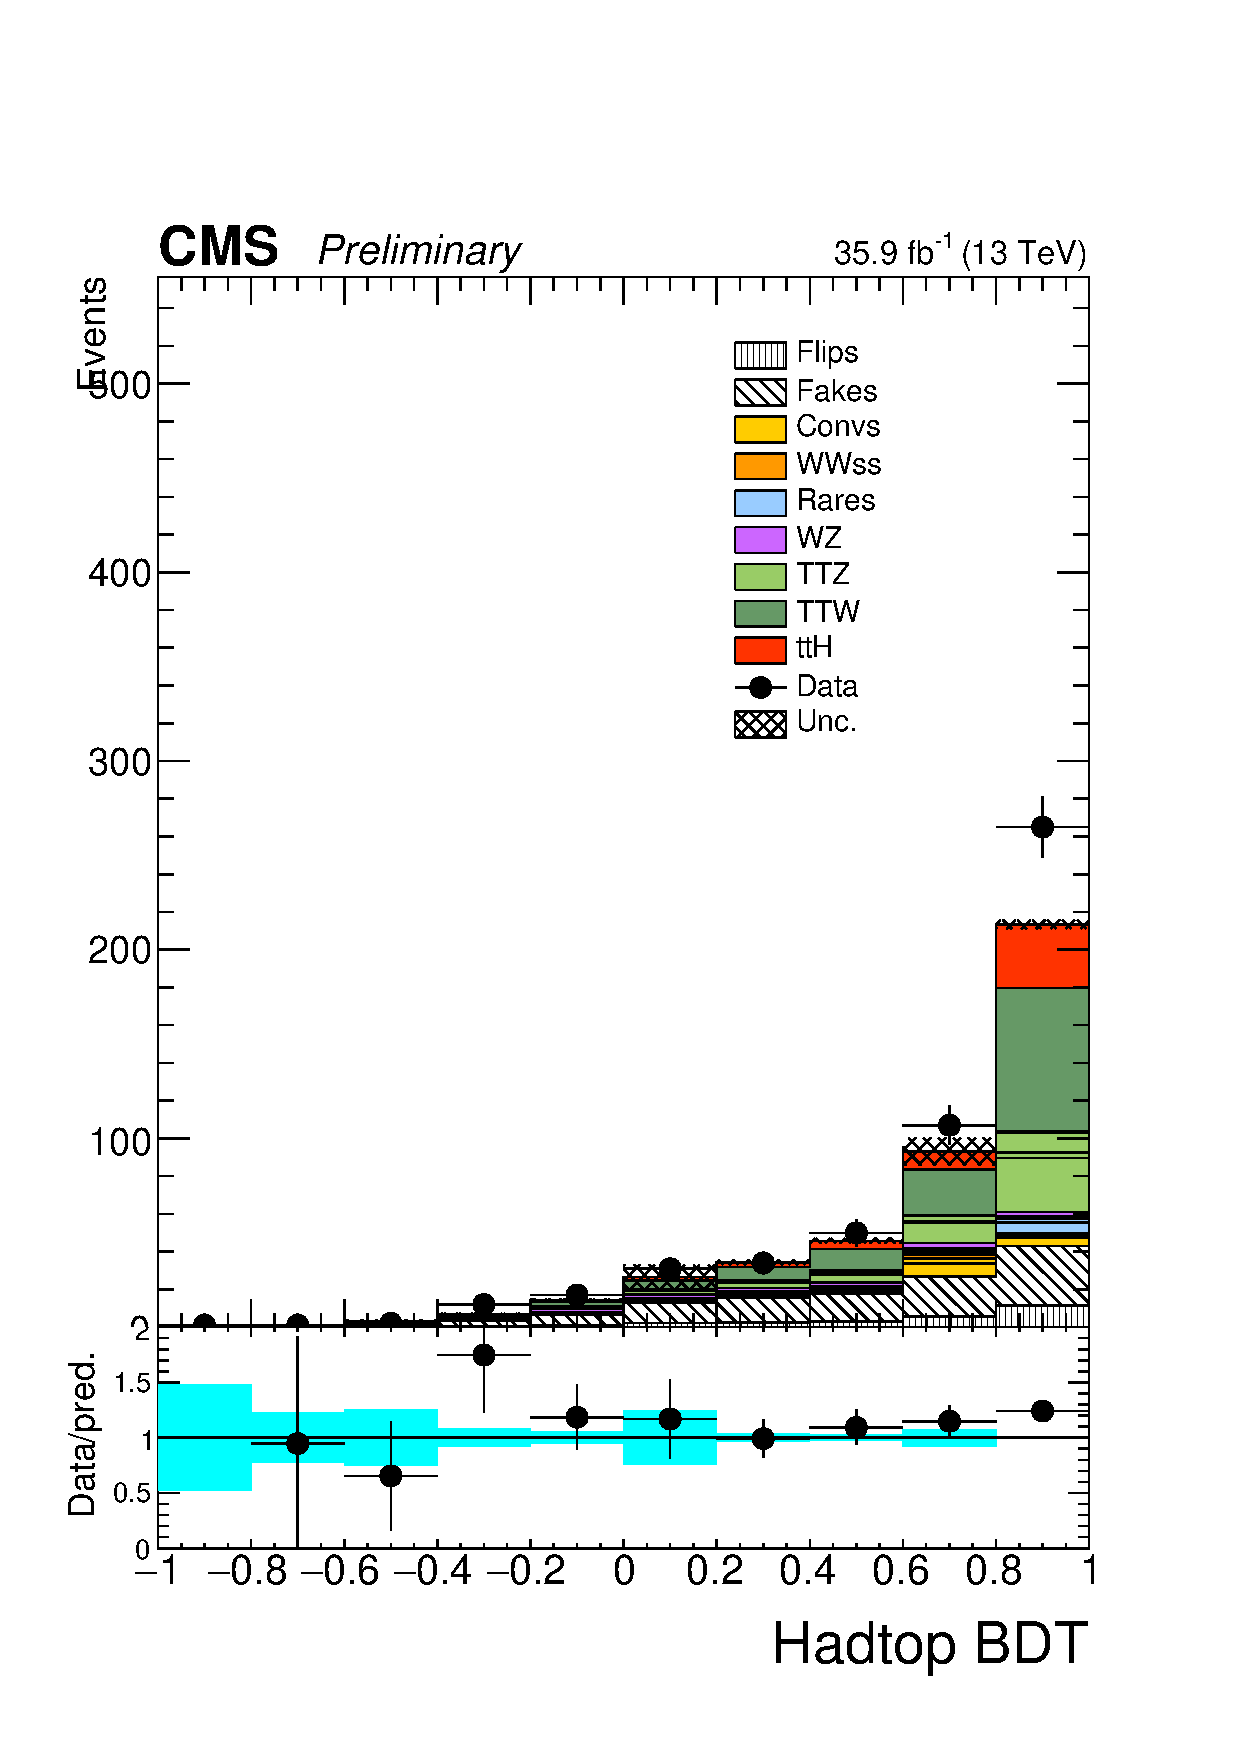
\includegraphics[width=0.49\textwidth]{ch9_figs/hadtop_bdt_ttH_stackPlot_SR.pdf}
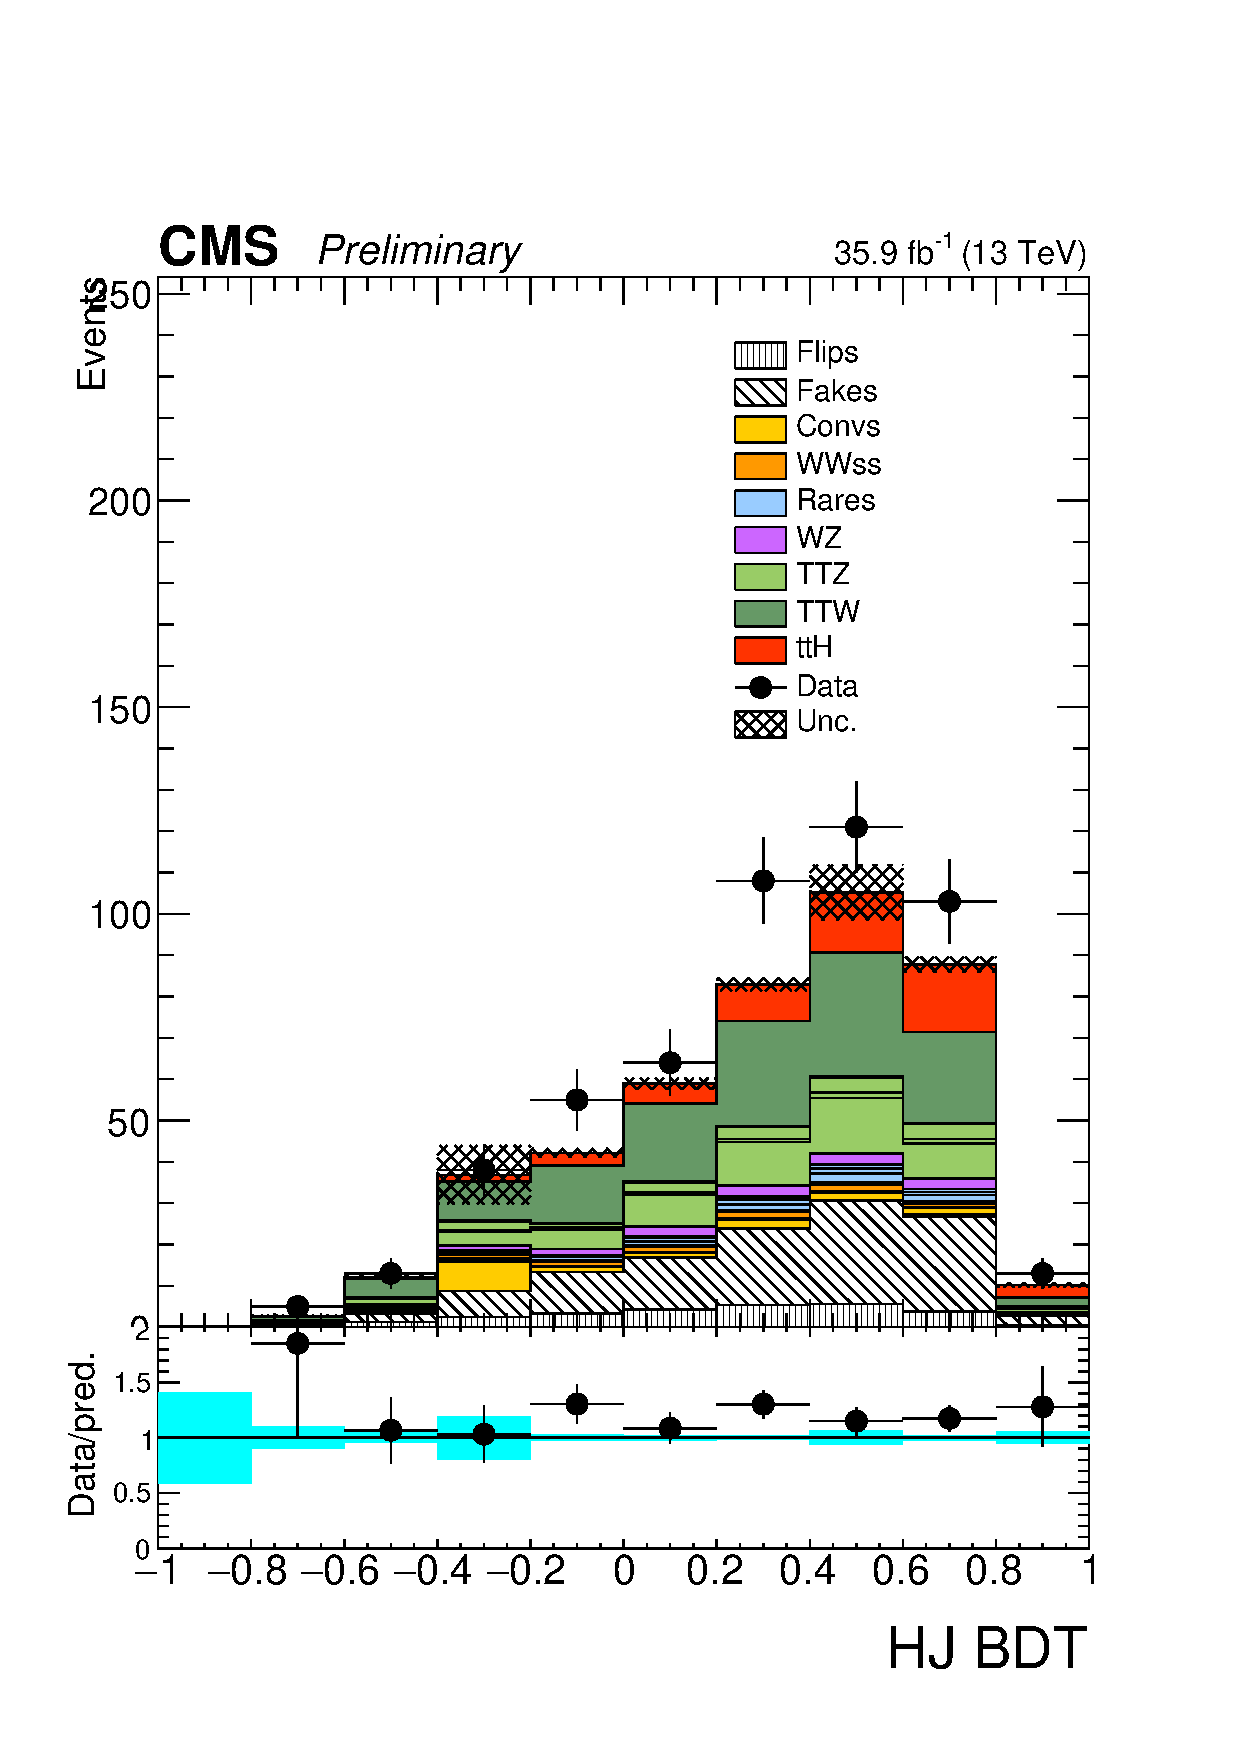
\includegraphics[width=0.49\textwidth]{ch9_figs/hj_bdt_ttH_stackPlot_SR.pdf}
\caption[Data to MC comparison of reconstruction BDT outputs]{The hadronic top BDT (left) and higgs tagger BDT (right) outputs.}
\label{fig:reco_bdt_stacks}
\end{figure}



\section{Binning}
The binning choice for the two-dimensional shape resulting from plotting each BDT on a separate axis is not straight forward, due to the large number of binning techniques
available. The binning method must optimally partition the space to isolate
signal from background, while simultaneously maintaining populated bins that don't suffer from low statistics. The output shapes formed by the two BDTs for the signal and largest backgrounds
are in Figure~\ref{fig:2d_shapes} below. 

\begin{figure}[htp]
\centering
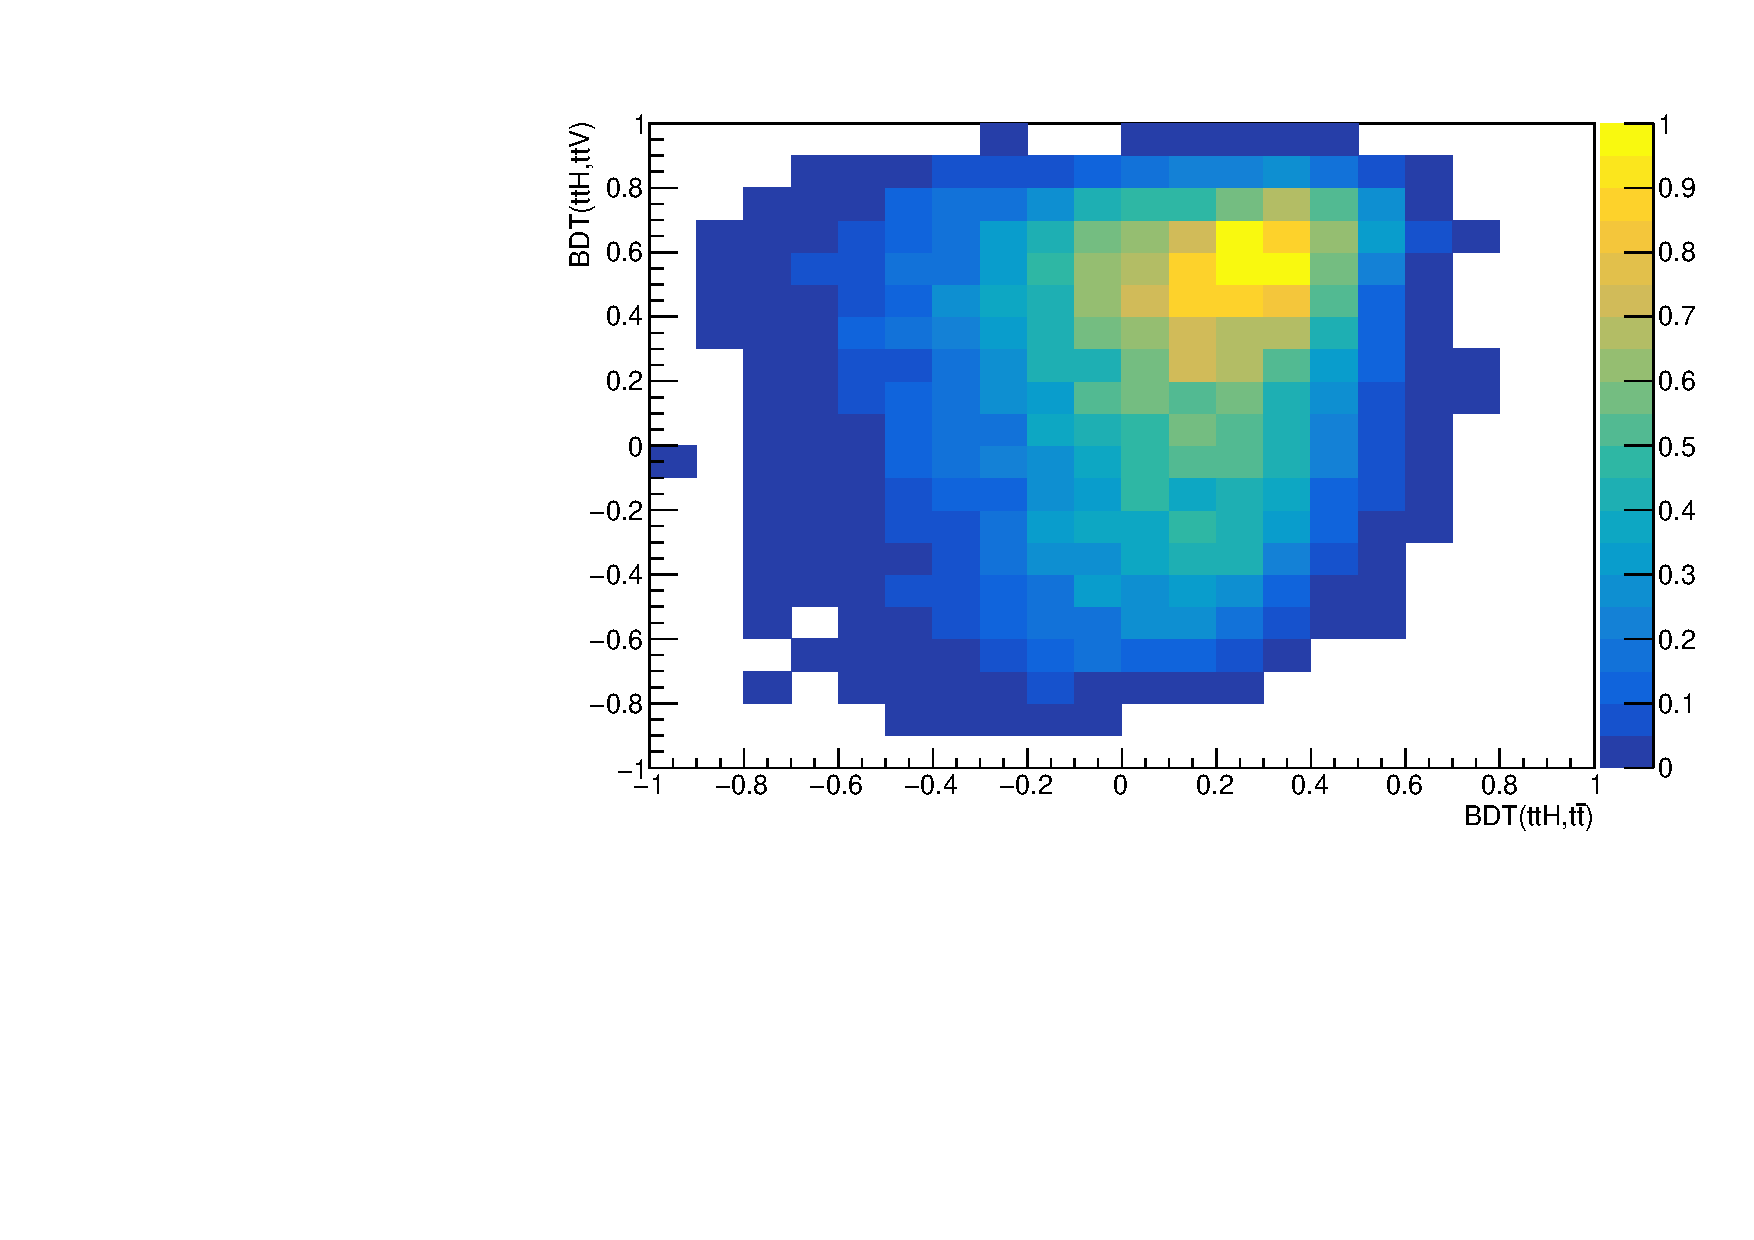
\includegraphics[width=0.49\textwidth]{ch9_figs/tth_2l_2D.pdf}\\
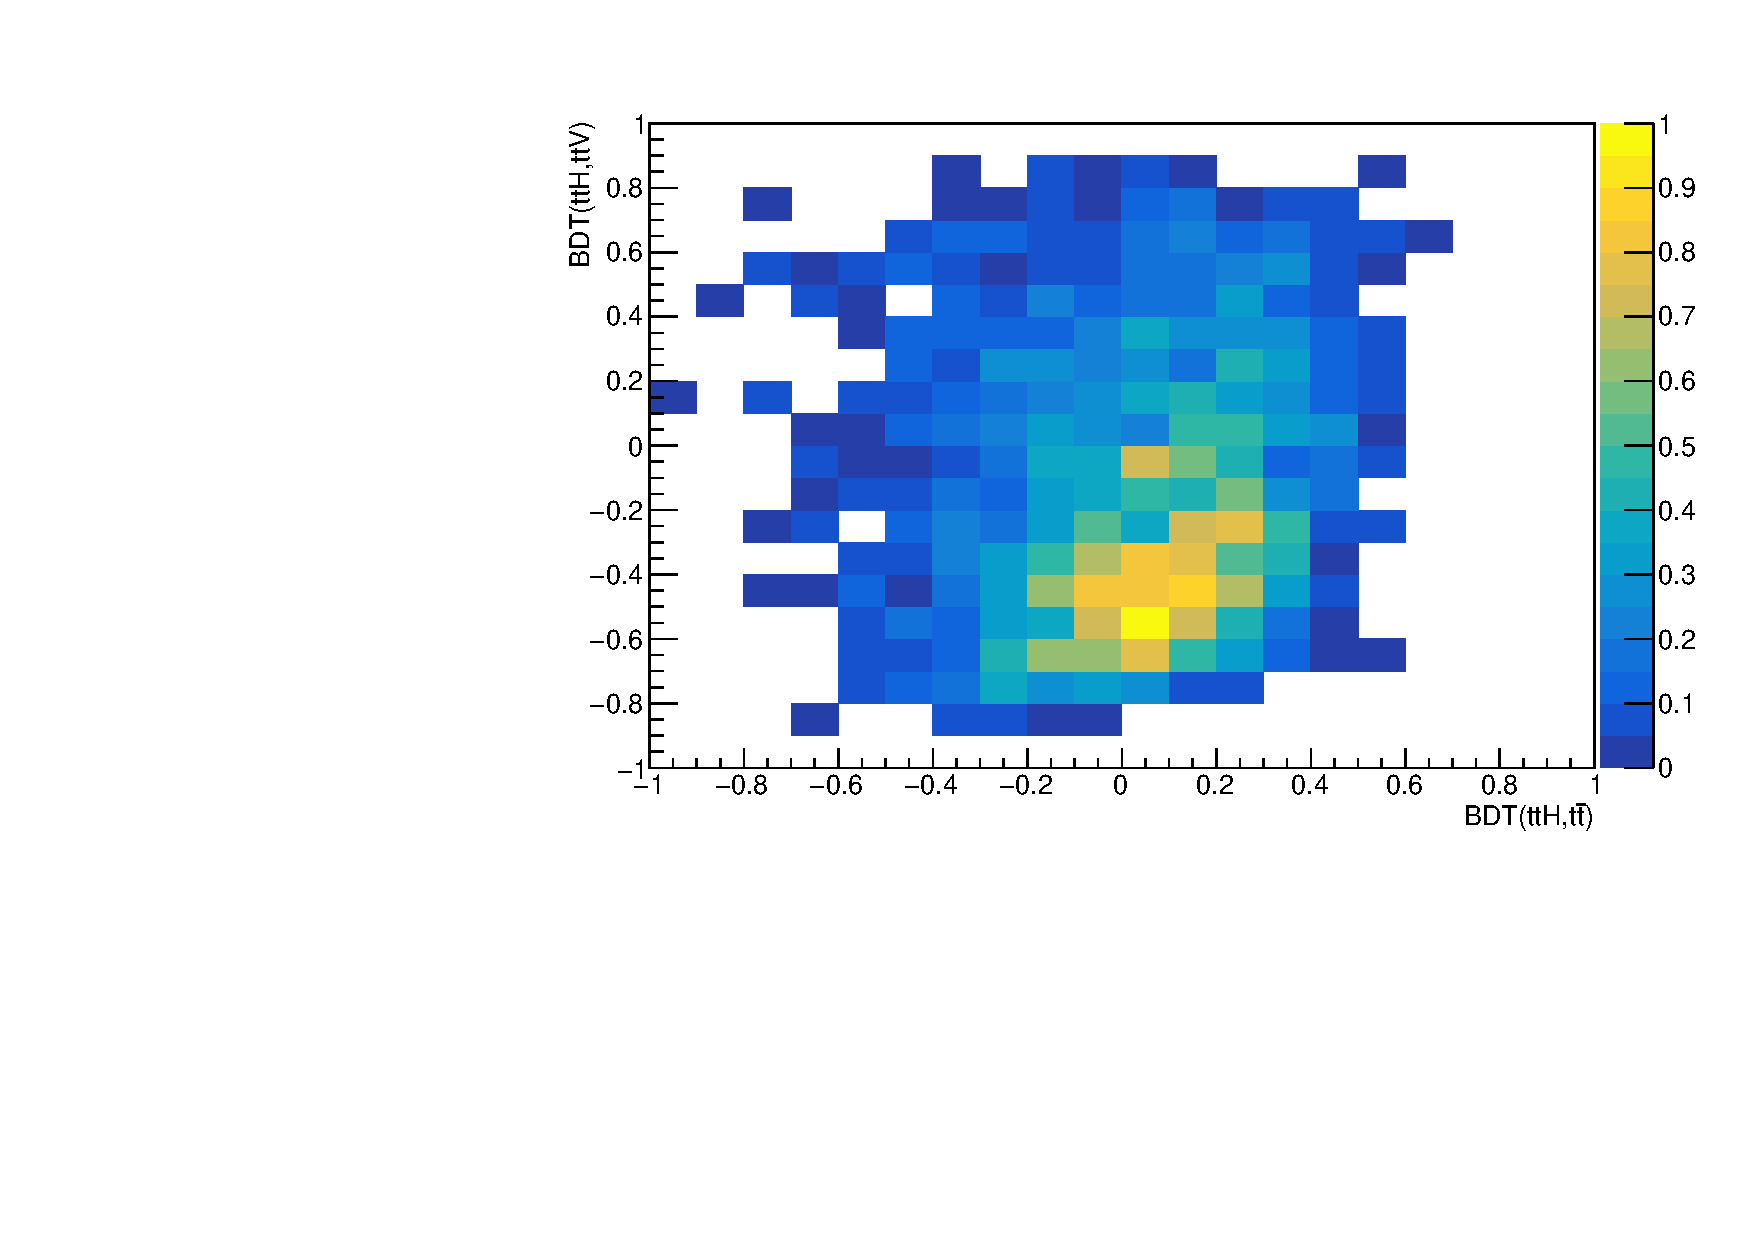
\includegraphics[width=0.49\textwidth]{ch9_figs/tt_2l_2D.pdf}
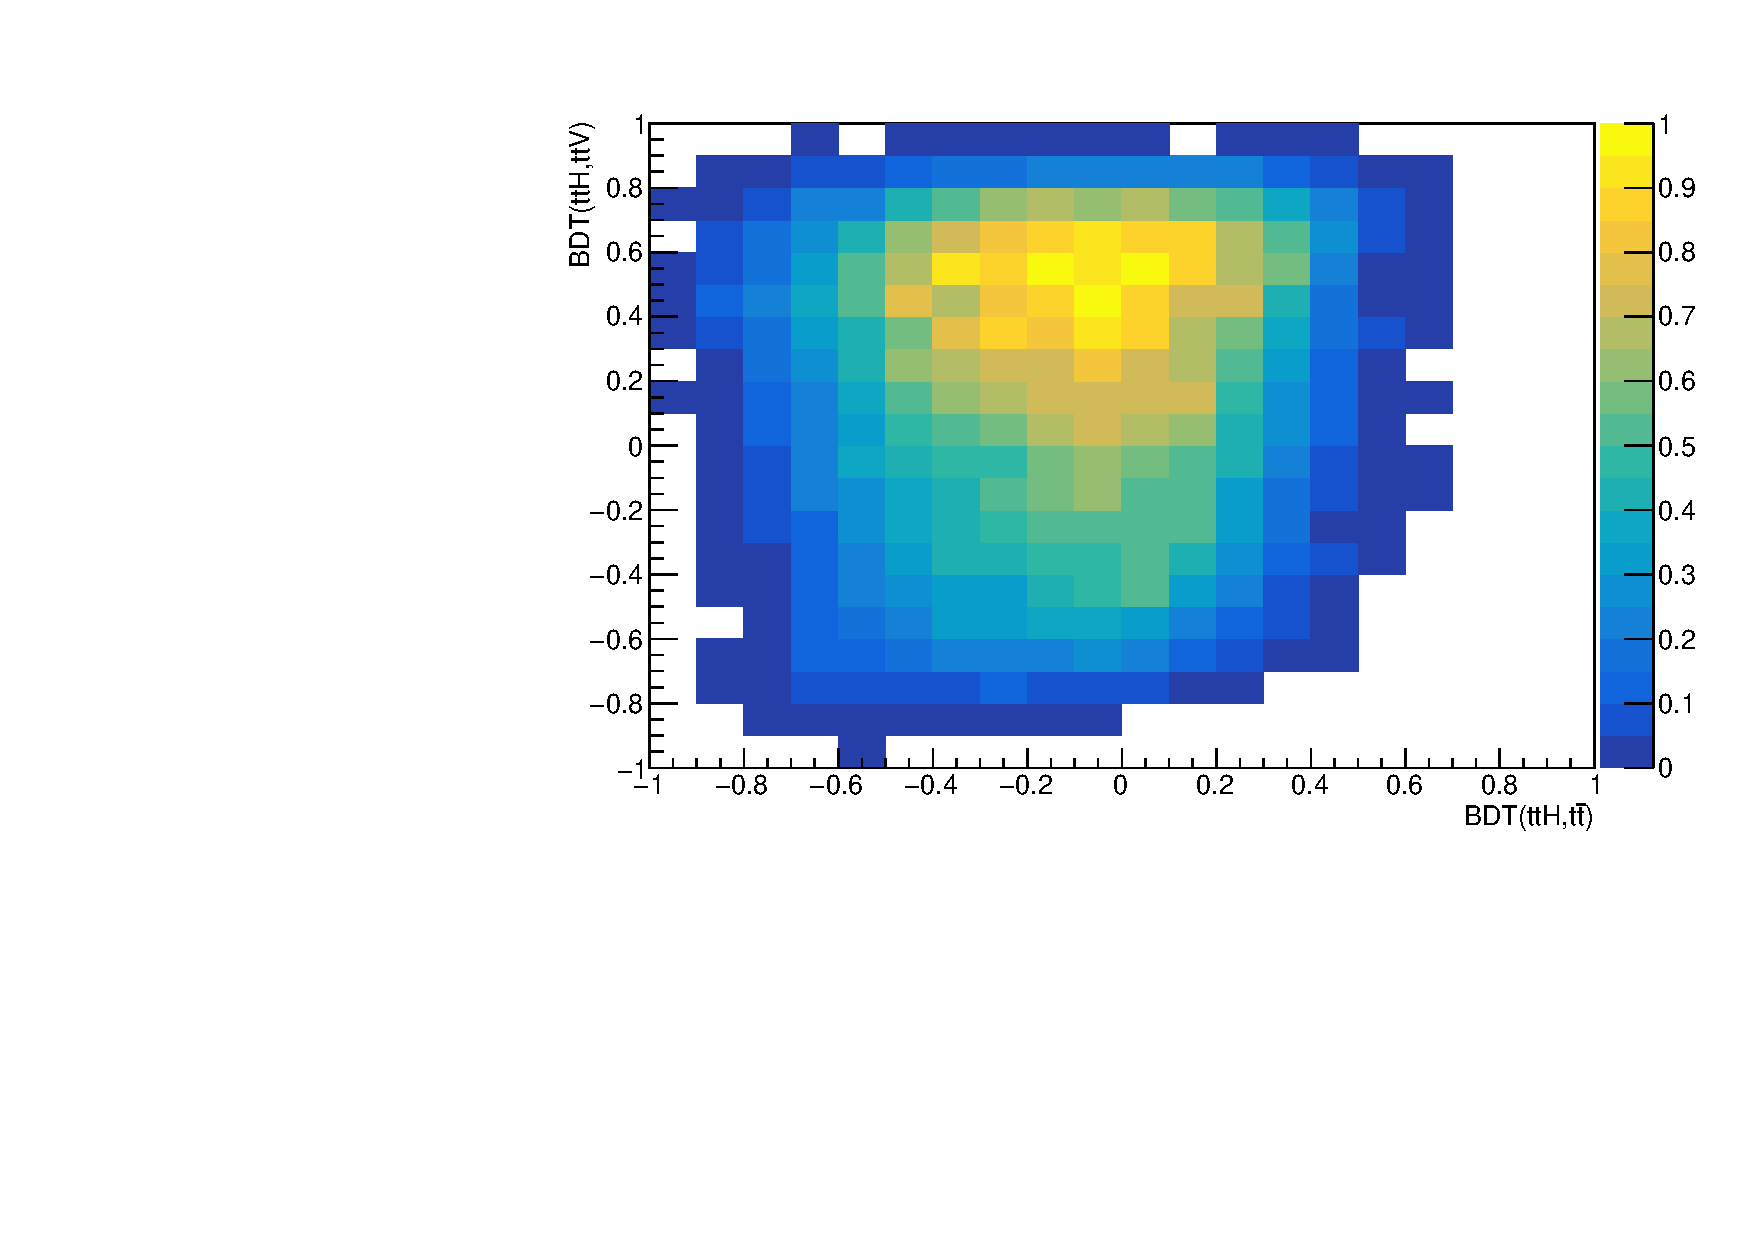
\includegraphics[width=0.49\textwidth]{ch9_figs/ttw_2l_2D.pdf}
\caption[Two dimensional BDT output shapes of signal and backgrounds]{The two-dimensional output shape formed by the two BDTs for \tth (top), \ttbar (left), and \ttv (right).}
\label{fig:2d_shapes}
\end{figure}

While previous versions of this analysis used a simple rectangular binning that was performed by studying the signal and background shapes and drawing the bins by hand,
this iteration takes a more algorithmic approach based on the signal-to-background likelihood ratio. The binning procedure was performed with signal and background MC that was not used
in the main analysis. The binning process begins with the standard rectangular, 20 x 20 binning in Figure~\ref{fig:2d_shapes}. For each bin, the signal to background likelihood ratio is computed.
Next, each background event from the \ttbar and \ttv samples is assigned the likelihood ratio corresponding to the bin it populates. The resulting likelihood distribution for background
events is transformed into the cumulative\footnote{A cumulative distribution function of some variable $S$, evaluated at $s$, is the probability that $S$ will have a value less than or equal
to $s$.} distribution below in Figure~\ref{fig:cum_dist} (left). The y-axis of the cumulative distribution function of background events is then binned evenly, achieving approximately equal
amounts of background in each bin.

\begin{figure}[htp]
\centering
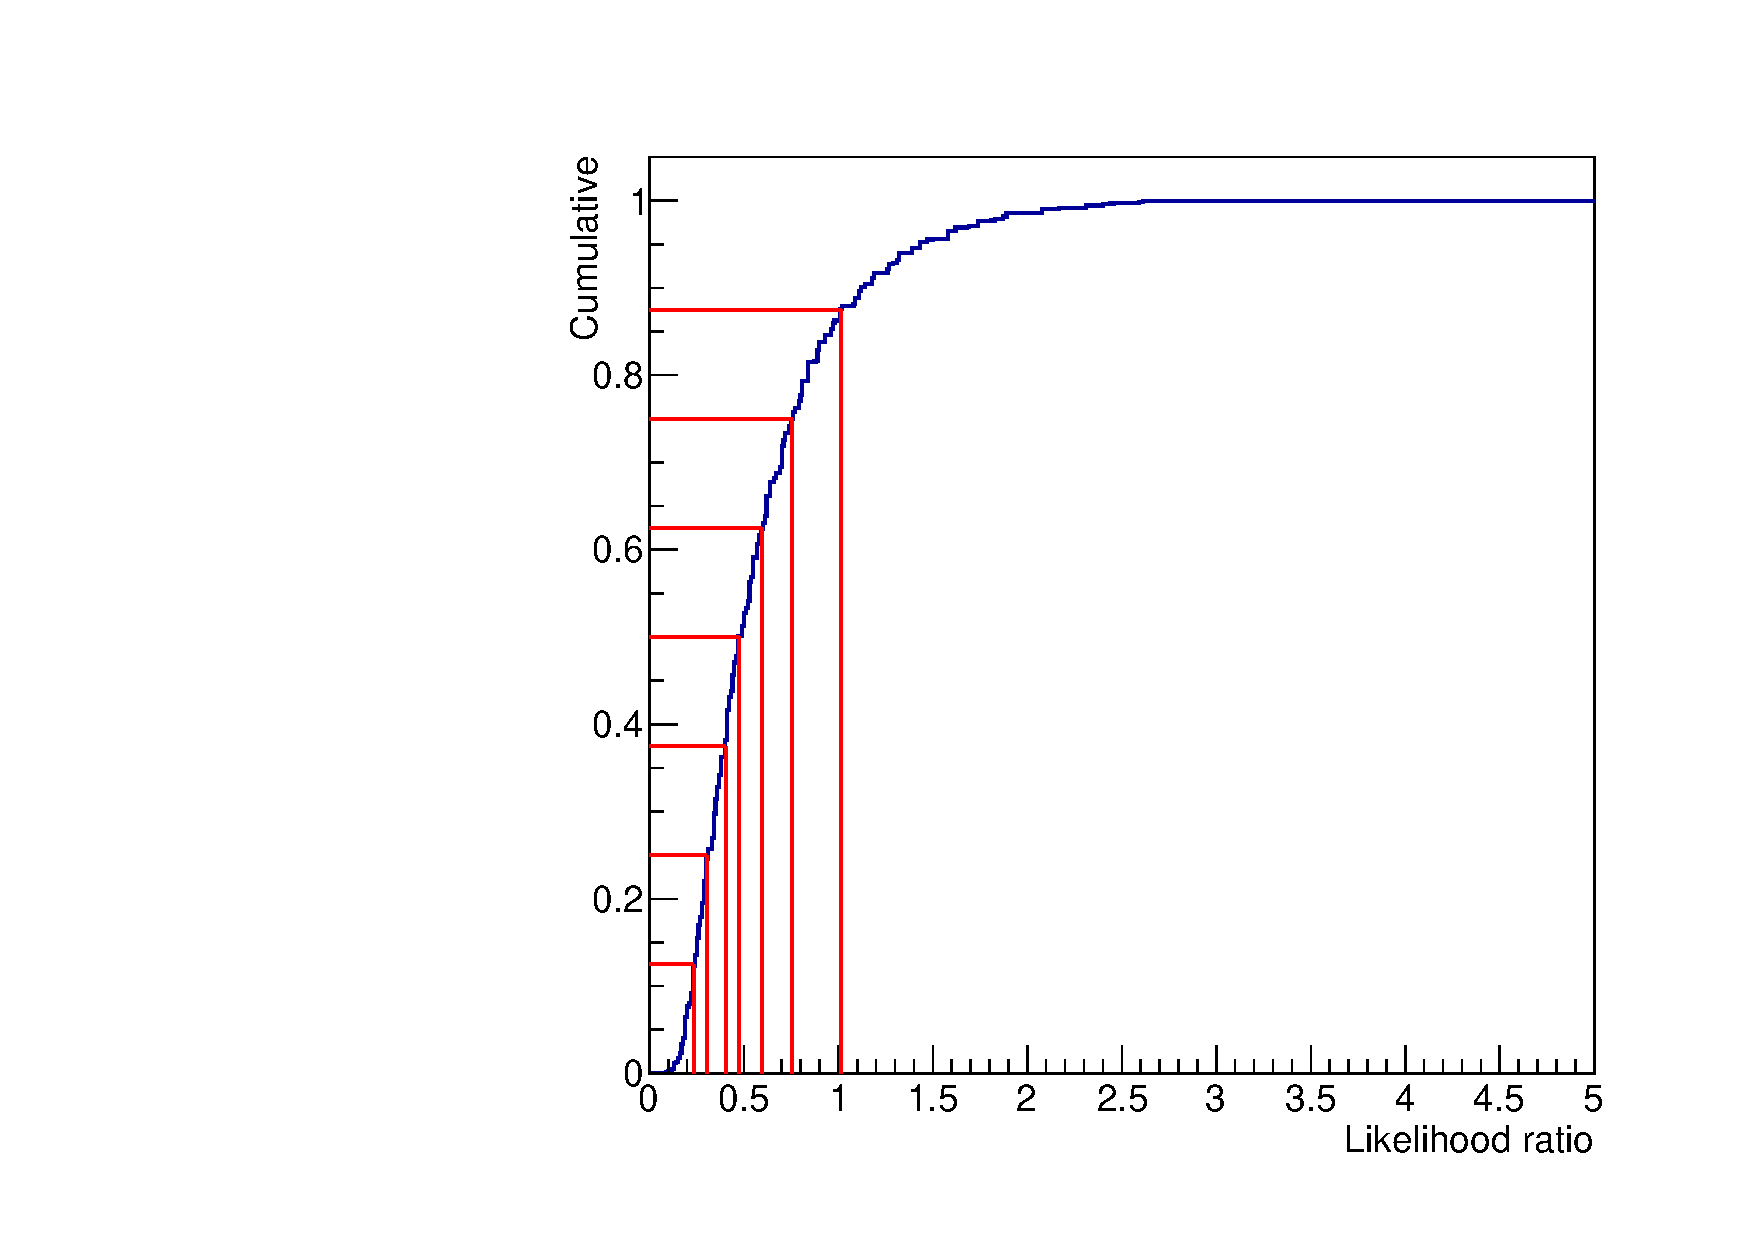
\includegraphics[width=0.49\textwidth]{ch9_figs/cumulative_2lss.pdf}
\caption[Cumulative distribution of signal-to-background likelihood ratio]{Cumulative distribution of signal-to-background likelihood ratio.}
\label{fig:cum_dist}
\end{figure}

\noindent The bins from the cumulative distribution are then mapped back to the 2D shape. This mapping is used as the final 2D binning and is represented in Figure~\ref{fig:likelihood} (left).
The corresponding 1D histogram resulting from this binning where the analysis is performed is Figure~\ref{fig:likelihood} (right). These bins are filled with separate signal and background
samples from the ones used for deriving final results. The choice of number of final bins is motived from a cross-check procedure based on the k-means algorithm, which yields similar
results~\cite{CMS-AN-17-029}. The pre-fit 1D shapes are in Figure~\ref{fig:final_shapes_prefit}. 

\begin{figure}[htp]
\centering
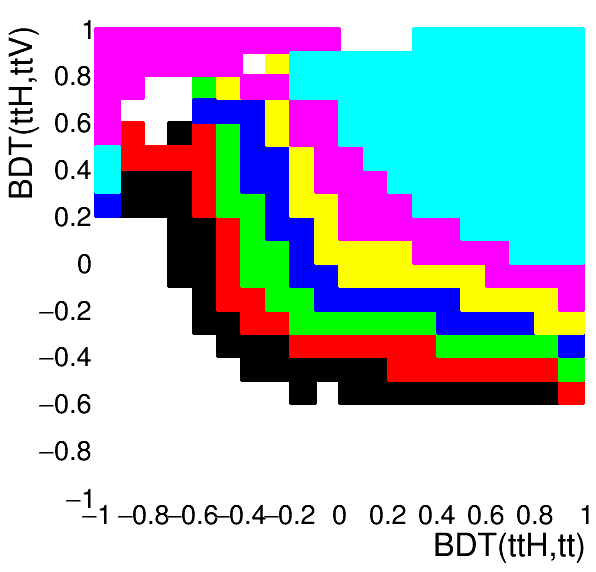
\includegraphics[width=0.49\textwidth]{ch9_figs/likelihoodBased_2d_2lss.png}
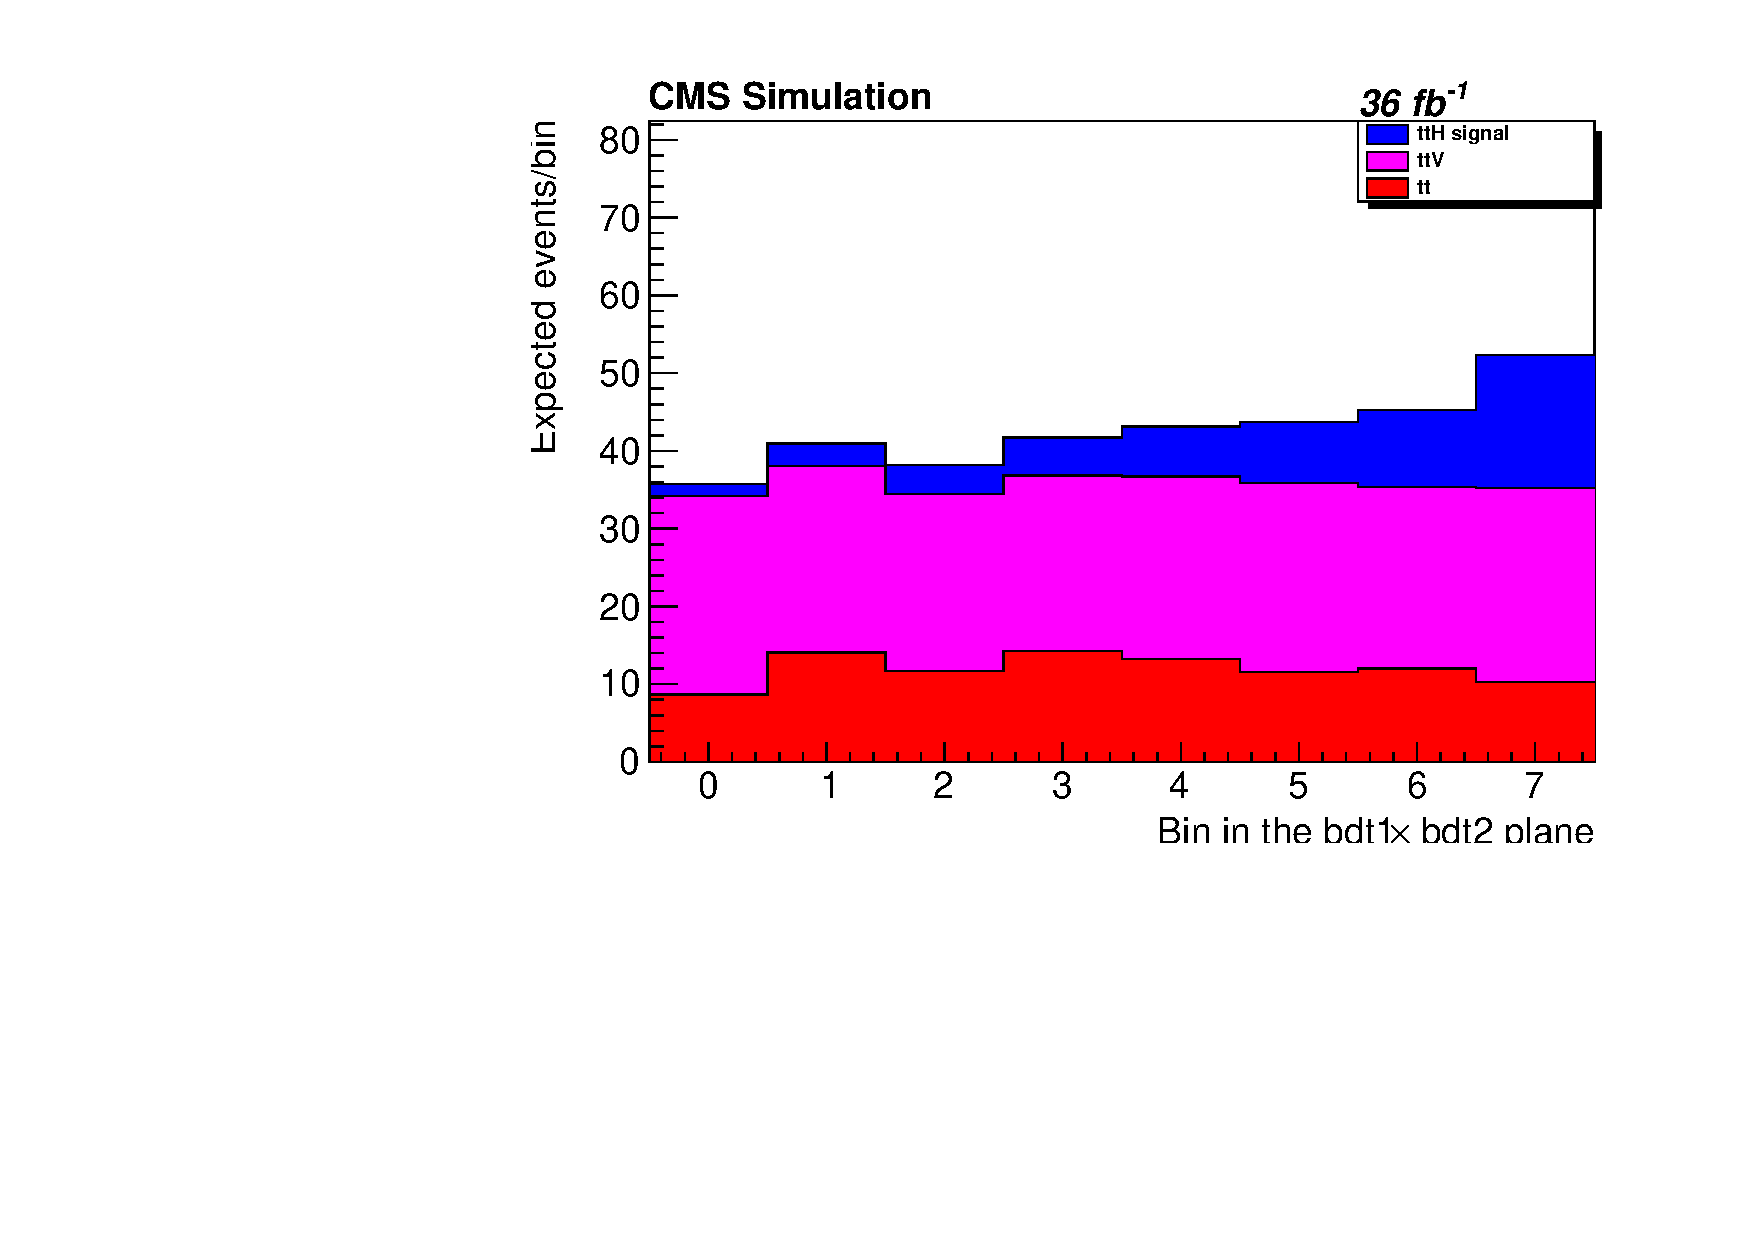
\includegraphics[width=0.49\textwidth]{ch9_figs/likelihoodBased_1d_2lss.pdf}
\caption[The 2D and 1D binning based on the cumulative likelihood distribution]{The 2D (left) and 1D (right) binning based on the cumulative likelihood distribution.
Each color on the 2D histogram corresponds to a bin on the 1D histogram, white-bin0, black-bin1, red-bin2, green-bin3, blue-bin4, yellow-bin5,pink-bin6, and cyan-bin7.}
\label{fig:likelihood}
\end{figure}

\begin{figure}[htp]
\centering
%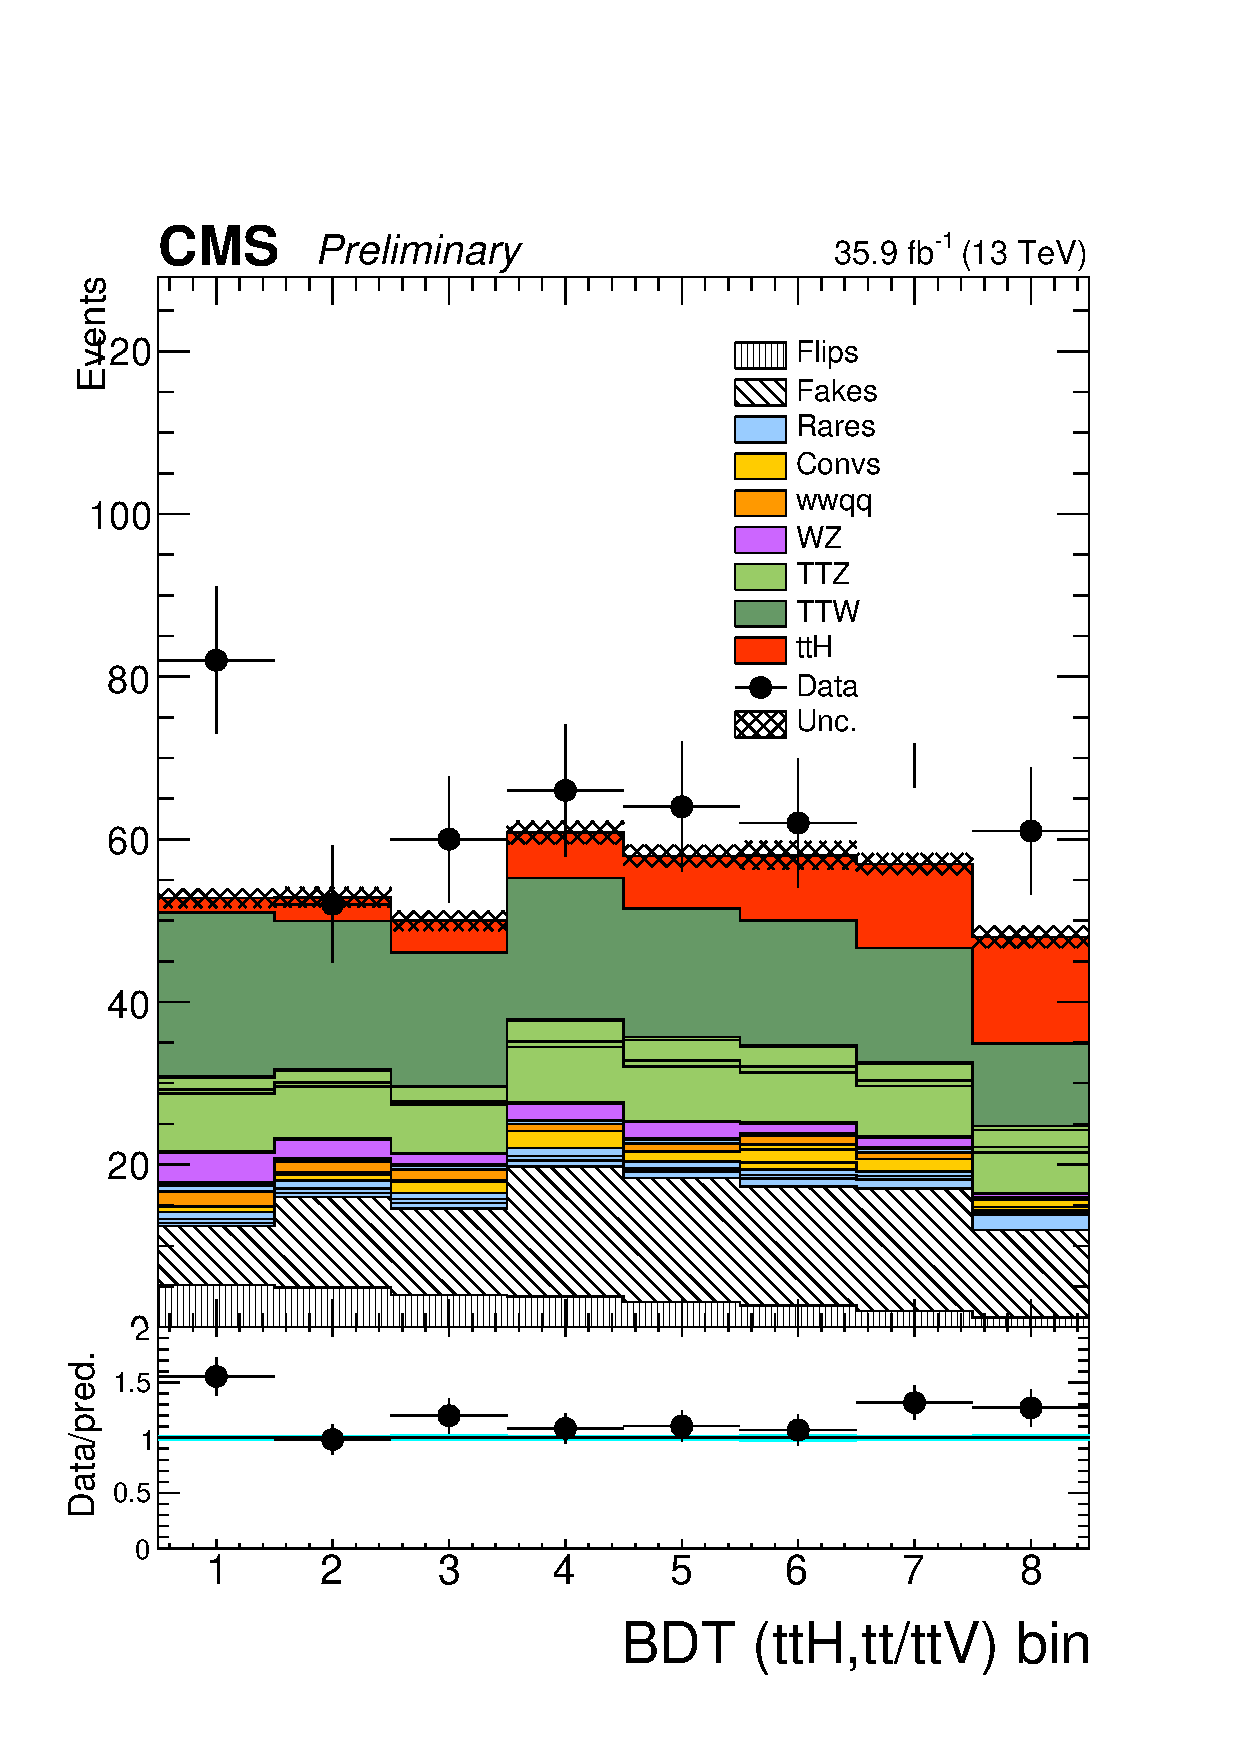
\includegraphics[width=0.49\textwidth]{ch9_figs/final_shape__ttH_stackPlot_SR.pdf}\\
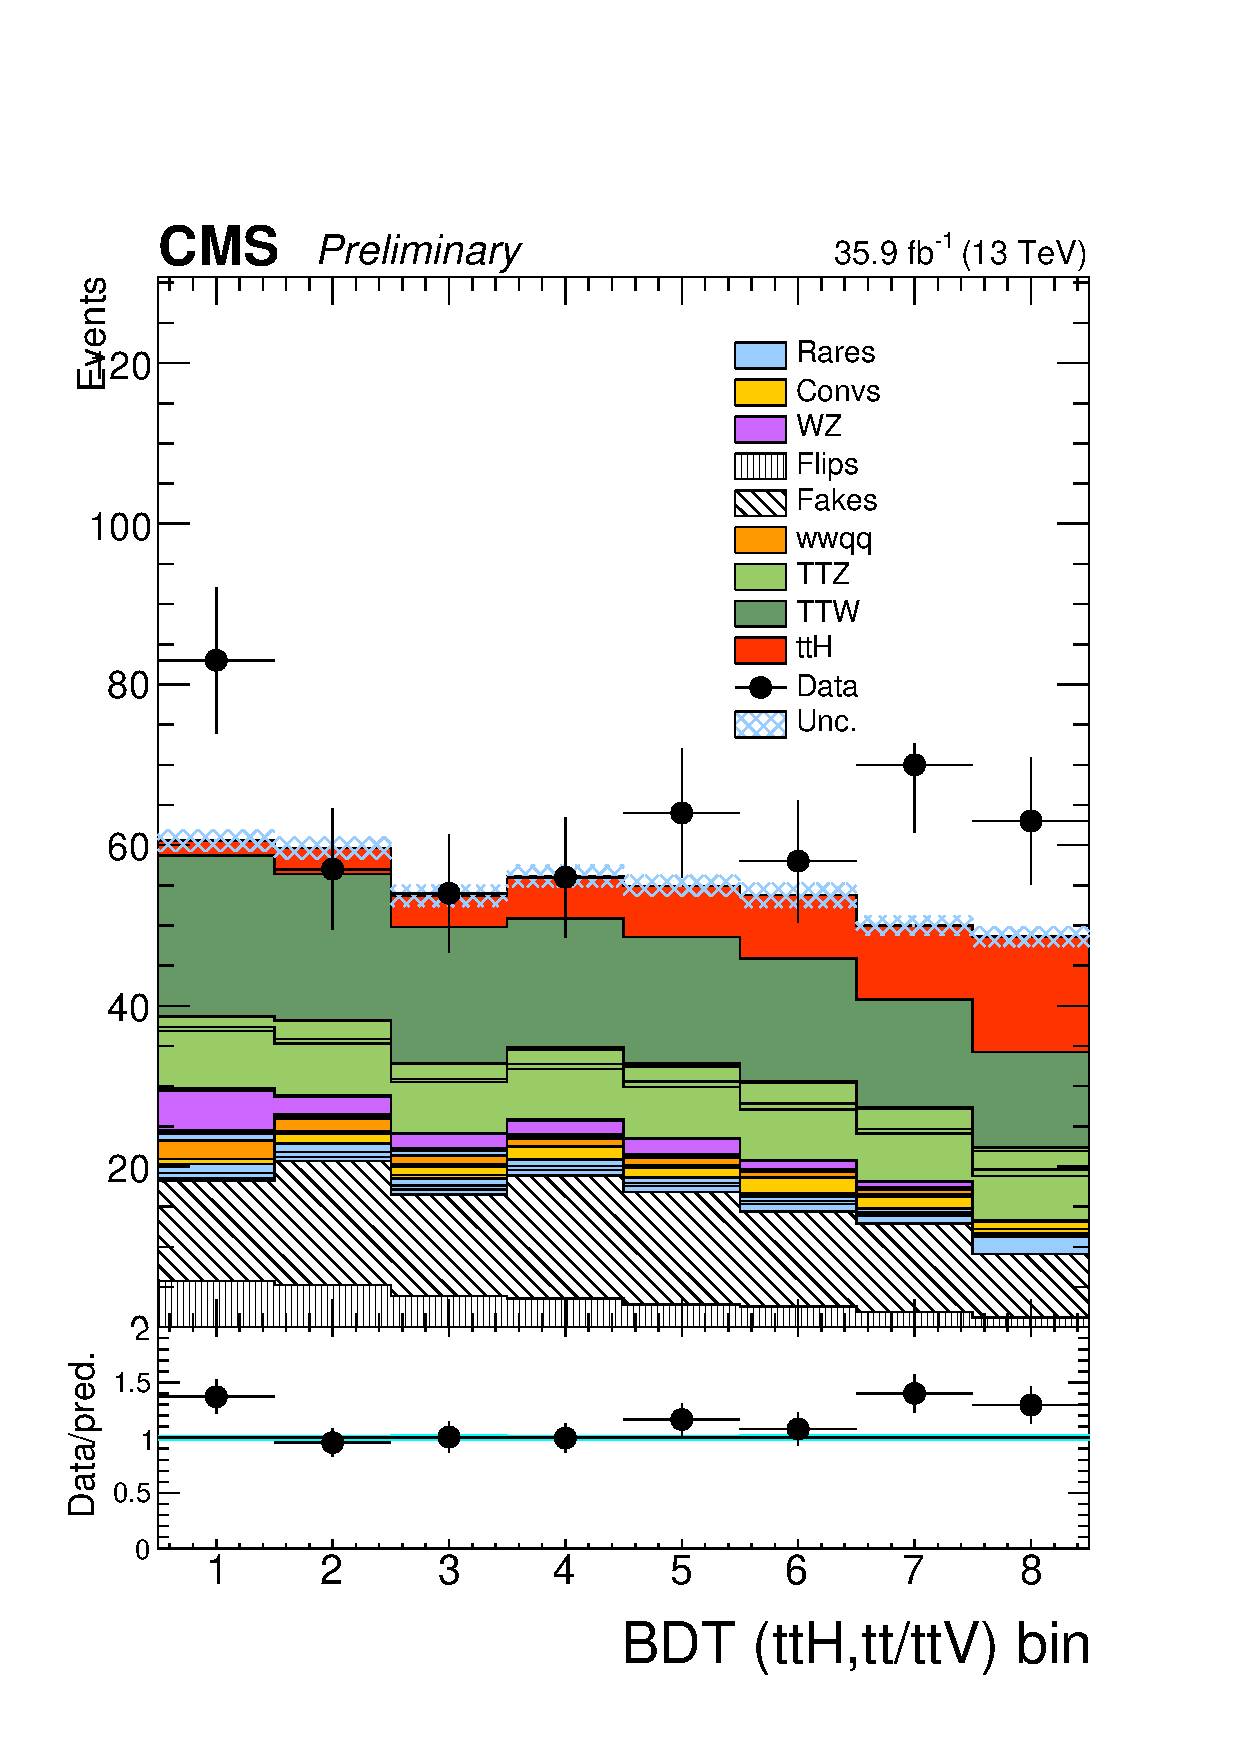
\includegraphics[width=0.49\textwidth]{ch9_figs/final_shape_bdtv8__ttH_stackPlot_SR.pdf}\\
%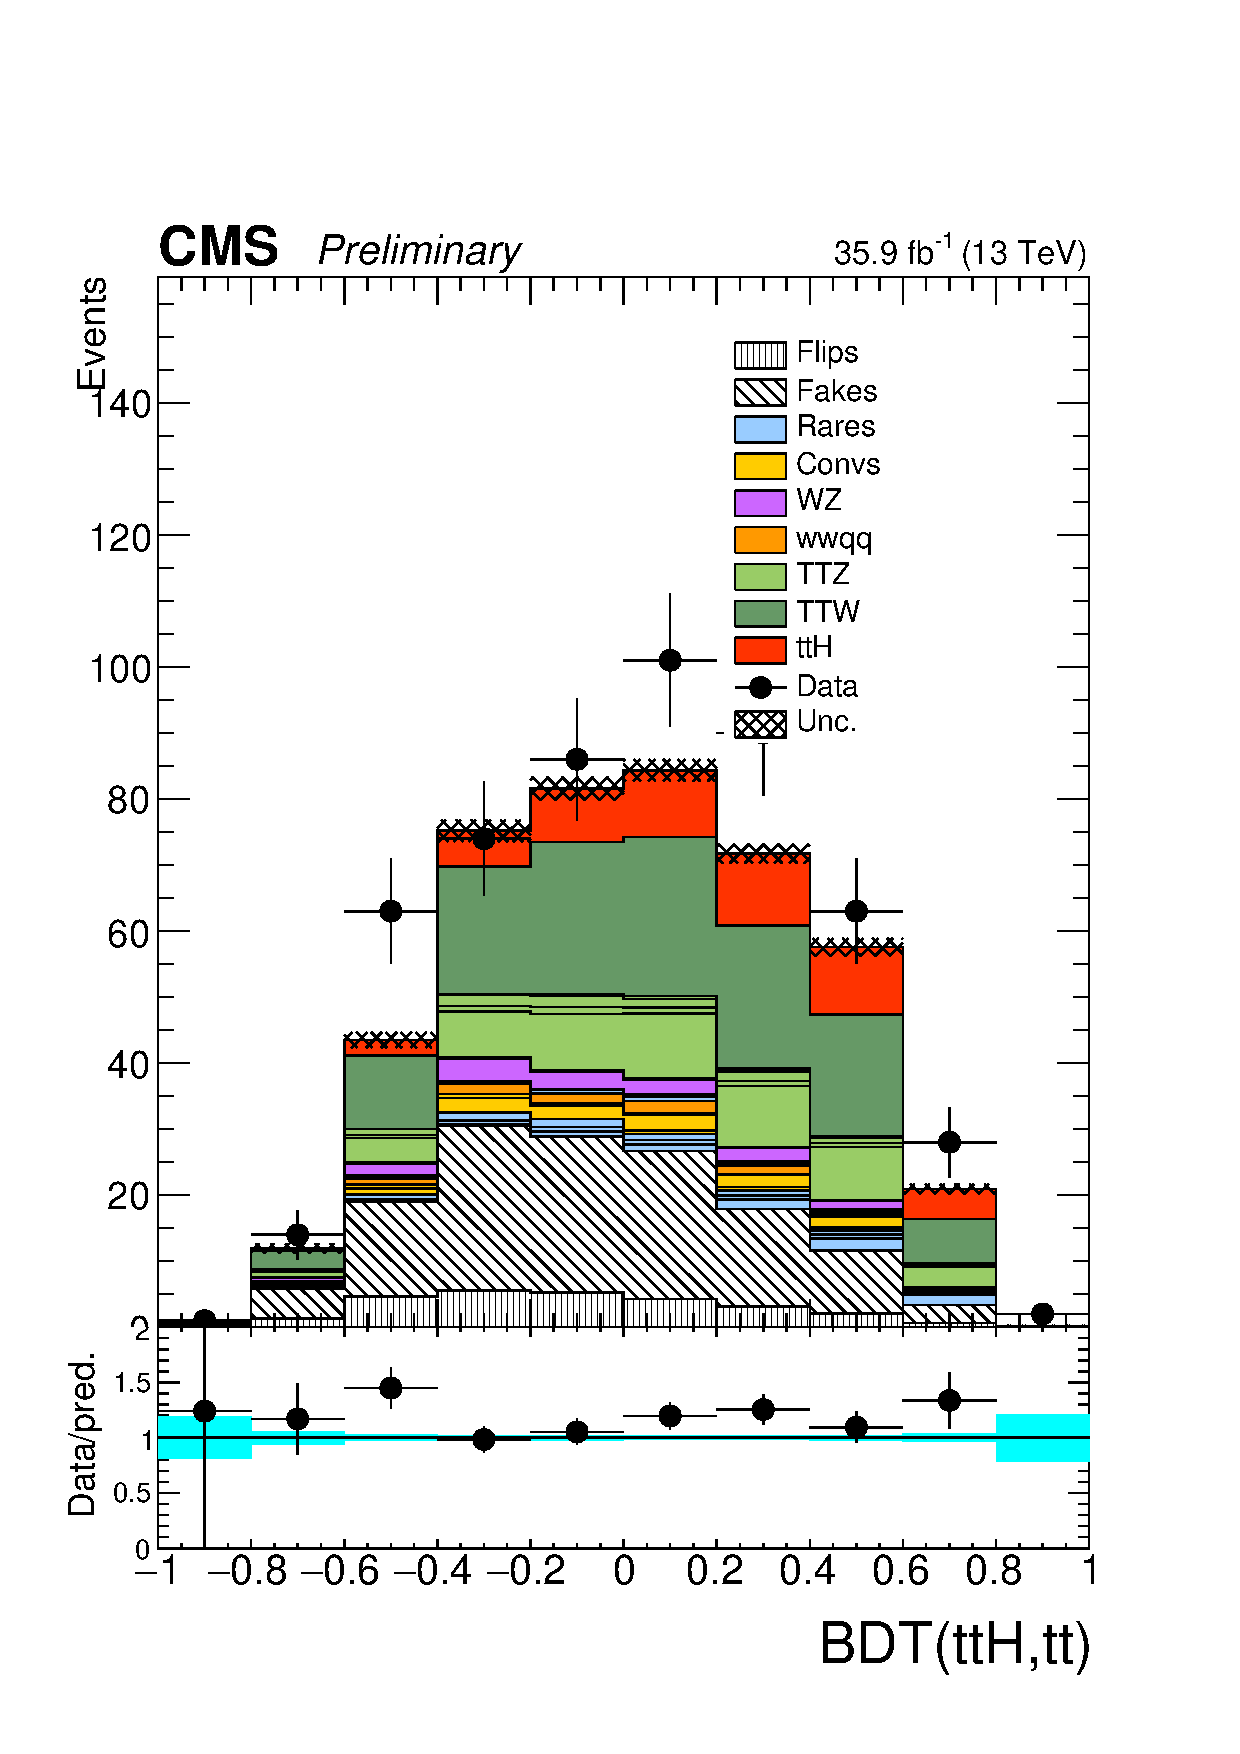
\includegraphics[width=0.49\textwidth]{ch9_figs/tt_BDT_ttH_stackPlot_SR.pdf}
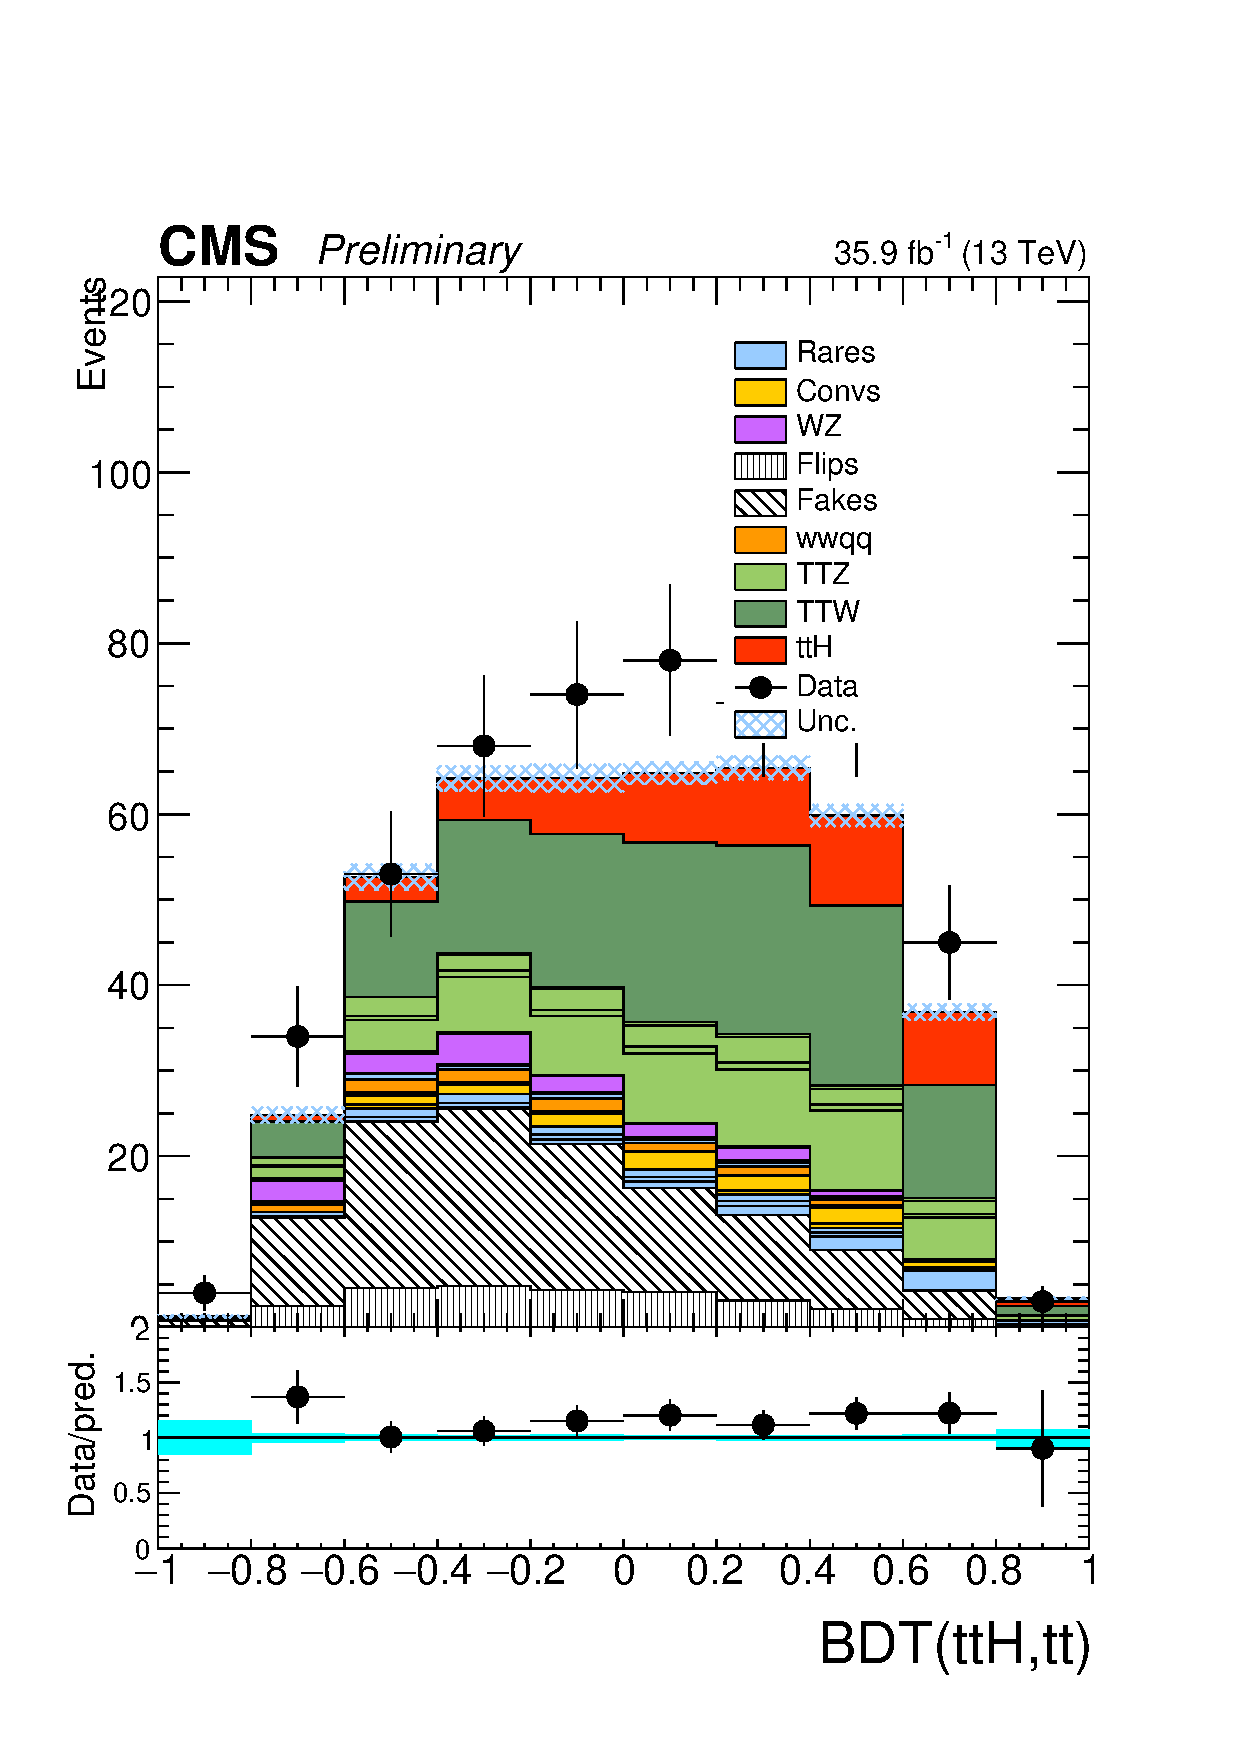
\includegraphics[width=0.49\textwidth]{ch9_figs/tt_BDT_BDTv8_ttH_stackPlot_SR.pdf}
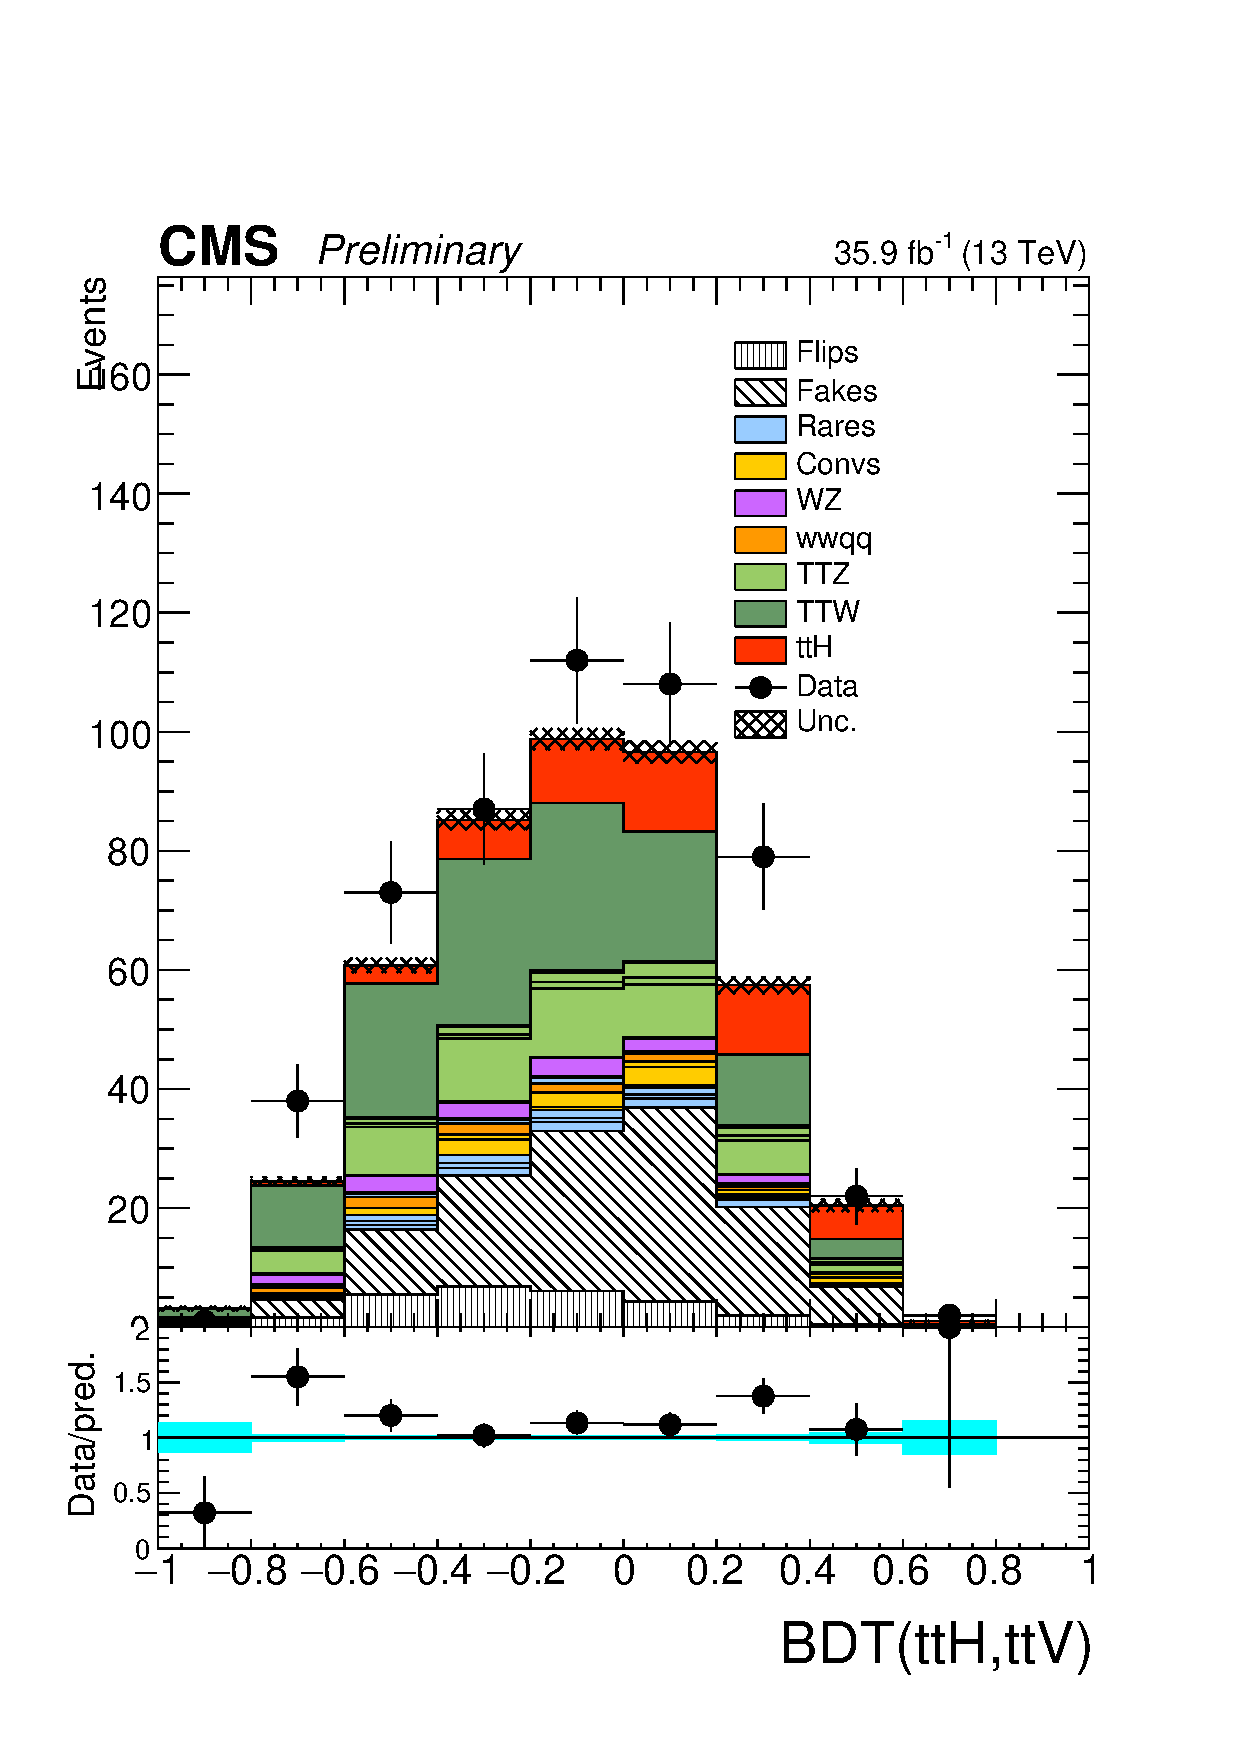
\includegraphics[width=0.49\textwidth]{ch9_figs/ttV_BDT_ttH_stackPlot_SR.pdf}
\caption[Data to MC comparison of final shapes]{The final 1D shape used for the analysis (top), the \ttbar BDT output (left) and the \ttv BDT output (right)}.
\label{fig:final_shapes_prefit}
\end{figure}


\section{Subcategorization}
In addition to the signal region categorization by lepton flavor, further categorization is applied to exploit differences between signal and background. All categories are
split by the sum of the lepton electric charges. This splitting helps to isolate the \ttw background, which is asymmetric in lepton charge sum because the initial state of the
diagram involves an incoming quark and antiquark. Because the LHC collides protons whose quark content is $uud$, this favors positively charged final states, while the \tth process
is initiated by gluon scattering, resulting in neutral final states, symmetric in lepton electric charge sum.
The signal region categories
are split further into two subcategories $b-tight$, which contains events with two b-jets passing the CSVv2 medium working point, and $b-loose$ which contains all other events
(those with fewer than 2 CSVv2 M jets). This splitting helps to separate \tth from the fake lepton background which is primarily comprised of \ttbar. Due to the same-sign 
lepton electric charge requirement, most of the \ttbar is vetoed, however there is a substantial amount of fakes originating from the b-decay. The b-jet is often removed
from the fake lepton in the jet cleaning step, described in Section~\ref{sec:cleaning}, while the fake lepton is kept. This produces events with a single b-jet, while \tth should more often have two b-jets. In total there are 10 categories
making up the signal region, illustrated in Figure~\ref{fig:subcats} below. The $ee$ channel is not split according to b-jet content due to low statistics. 
It is the final shapes in these subcategories that are used for the final tabulation of signal, background, and data. 

\begin{figure}[htp]
\centering
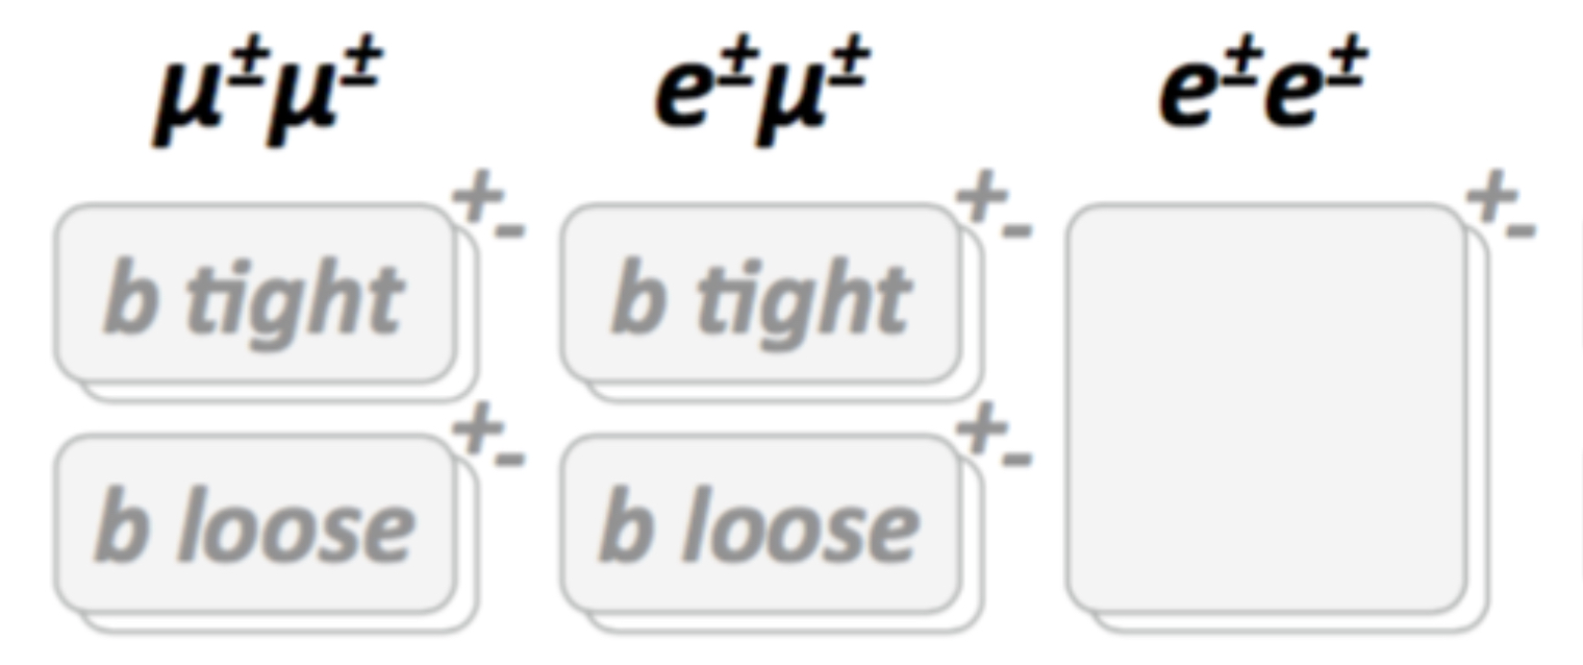
\includegraphics[width=0.7\textwidth]{ch9_figs/subcats.pdf}
\caption[Sub categories used for signal extraction]{The 10 subcategories used for signal extraction.}
\label{fig:subcats}
\end{figure}


